\documentclass[10pt,a4paper,twoside]{book}

% TODO: among us

%%%%%%%%%%%%%%%%%%%%%%%%%%%%%%%%%%%%%%%%%
% Template Dispense
% Autore: Teo Bucci
%%%%%%%%%%%%%%%%%%%%%%%%%%%%%%%%%%%%%%%%%

%---------------------------
% FONTS AND LANGUAGE
%---------------------------

\usepackage[T1]{fontenc}
\usepackage[utf8]{inputenc}
\usepackage[english]{babel}

%---------------------------
% PACKAGES
%---------------------------

\usepackage{dsfont} % for using \mathds{1} characteristic function
\usepackage{amsmath, amssymb, amsthm} % amssymb also loads amsfonts
\usepackage{latexsym}
\usepackage{comment}

\usepackage{booktabs}
\usepackage{pgfplots}
\usepackage{tikz}
\usetikzlibrary{
  positioning,
  shapes.misc,
  intersections,
  shapes.symbols,
  patterns,
  fadings,
  shadows.blur,
  decorations.pathreplacing,
  arrows.meta,
  arrows
}
\usepackage{mathdots}
\usepackage{cancel}
\usepackage{color}
\usepackage{siunitx}
\usepackage{array}
\usepackage{multirow}
\usepackage{makecell}
\usepackage{tabularx}
\usepackage{caption}
\usepackage{subcaption}
\captionsetup{belowskip=12pt,aboveskip=4pt}
\usepackage{subcaption}
\usepackage{placeins} % \FloatBarrier
\usepackage{flafter}  % The flafter package ensures that floats don't appear until after they appear in the code.
\usepackage[shortlabels]{enumitem}
\usepackage[english]{varioref}
\renewcommand{\ref}{\vref}

%---------------------------
% INCLUSIONE FIGURE
%---------------------------

\usepackage{import}
\usepackage{pdfpages}
\usepackage{transparent}
\usepackage{xcolor}
\usepackage{graphicx}
\graphicspath{ {./images/} } % Path relative to the main .tex file
\usepackage{float}

\newcommand{\fg}[3][\relax]{%
  \begin{figure}[H]%[htp]%
    \centering
    \captionsetup{width=0.7\textwidth}
      \includegraphics[width = #2\textwidth]{#3}%
      \ifx\relax#1\else\caption{#1}\fi
      \label{#3}
  \end{figure}%
  \FloatBarrier%
}

%---------------------------
% PARAGRAPHS AND LINES
%---------------------------

\usepackage[none]{hyphenat} % no hyphenation

\emergencystretch 3em % to prevent the text from going beyond margins

\usepackage[skip=0.2\baselineskip+2pt]{parskip}

% \renewcommand{\baselinestretch}{1.5} % line spacing

%---------------------------
% HEADERS AND FOOTERS
%---------------------------

\usepackage{fancyhdr}

\fancypagestyle{toc}{%
\fancyhf{}%
\fancyfoot[C]{\thepage}%
\renewcommand{\headrulewidth}{0pt}%
\renewcommand{\footrulewidth}{0pt}
}

\fancypagestyle{fancy}{%
\fancyhf{}%
\fancyhead[RE]{\nouppercase{\leftmark}}%
\fancyhead[LO]{\nouppercase{\rightmark}}%
\fancyhead[LE,RO]{\thepage}%
\renewcommand{\footrulewidth}{0pt}%
\renewcommand{\headrulewidth}{0.4pt}
}

% Removes the header from odd empty pages at the end of chapters
\makeatletter
\renewcommand{\cleardoublepage}{
\clearpage\ifodd\c@page\else
\hbox{}
\vspace*{\fill}
\thispagestyle{empty}
\newpage
\fi}

%---------------------------
% CUSTOM
%---------------------------

\usepackage{xspace}
\newcommand{\latex}{\LaTeX\xspace}
\newcommand{\tex}{\TeX\xspace}

\newcommand{\Tau}{\mathcal{T}}
\newcommand{\Ind}{\mathds{1}} % indicatrice

\newcommand{\transpose}{^{\mathrm{T}}}
\newcommand{\complementary}{^{\mathrm{C}}} % alternative ^{\mathrm{C}} ^{\mathrm{c}} ^{\mathsf{c}}
\newcommand{\degree}{^\circ\text{C}} % simbolo gradi

\newcommand{\notimplies}{\mathrel{{\ooalign{\hidewidth$\not\phantom{=}$\hidewidth\cr$\implies$}}}}
\newcommand{\questeq}{\overset{?}{=}} % è vero che?

\newcommand{\indep}{\perp \!\!\! \perp} % indipendenza
\newcommand{\iid}{\stackrel{\mathrm{iid}}{\sim}}
\newcommand{\event}[1]{\emph{``#1''}} % evento

% variazioni del simbolo "="
\newcommand{\iideq}{\overset{\text{\tiny iid}}{=}}
\newcommand{\ideq}{\overset{\text{\tiny id}}{=}}
\newcommand{\indepeq}{\overset{\perp \!\!\! \perp}{=}}

\newcommand{\boxedText}[1]{\noindent\fbox{\parbox{\textwidth}{#1}}}

\renewcommand{\emptyset}{\varnothing}
\renewcommand{\tilde}{\widetilde}
\renewcommand{\hat}{\widehat}

\DeclareMathOperator{\sgn}{sgn}
\DeclareMathOperator{\Var}{Var}
\DeclareMathOperator{\Cov}{Cov}
\DeclareMathOperator*{\rank}{rank}
\DeclareMathOperator*{\eig}{eig}
\DeclareMathOperator{\tr}{tr}
\DeclareMathOperator{\Grad}{grad}
\DeclareMathOperator{\Div}{div}
\DeclareMathOperator{\Span}{span}
\let\Im\undefined  % redefine \Im
\DeclareMathOperator{\Im}{Im}
\DeclareMathOperator{\Ker}{Ker}
\DeclareMathOperator*{\argmin}{arg\,min}
\DeclareMathOperator*{\argmax}{arg\,max}
\DeclareMathOperator*{\esssup}{ess\ sup}
\DeclareMathOperator*{\essinf}{ess\ inf}
\DeclareMathOperator*{\supp}{supp}

\newcommand{\eps}{\varepsilon}

\usepackage{mathtools} % Serve per i comandi dopo
\DeclarePairedDelimiter{\abs}{\lvert}{\rvert} % absolute value
\DeclarePairedDelimiter{\norm}{\lVert}{\rVert} % norm
\DeclarePairedDelimiter{\sca}{\langle}{\rangle} % scalar product

% Bold
\renewcommand{\AA}{\mathbb A}
\newcommand{\BB}{\mathbb{B}}
\newcommand{\CC}{\mathbb{C}}
\newcommand{\DD}{\mathbb{D}}
\newcommand{\EE}{\mathbb{E}}
\newcommand{\FF}{\mathbb{F}}
\newcommand{\GG}{\mathbb{G}}
\newcommand{\HH}{\mathbb{H}}
\newcommand{\II}{\mathbb{I}}
\newcommand{\JJ}{\mathbb{J}}
\newcommand{\KK}{\mathbb{K}}
\newcommand{\LL}{\mathbb{L}}
\newcommand{\MM}{\mathbb{M}}
\newcommand{\NN}{\mathbb{N}}
\newcommand{\OO}{\mathbb{O}}
\newcommand{\PP}{\mathbb{P}}
\newcommand{\QQ}{\mathbb{Q}}
\newcommand{\RR}{\mathbb{R}}
\renewcommand{\SS}{\mathbb S}
\newcommand{\TT}{\mathbb{T}}
\newcommand{\UU}{\mathbb{U}}
\newcommand{\VV}{\mathbb{V}}
\newcommand{\WW}{\mathbb{W}}
\newcommand{\XX}{\mathbb{X}}
\newcommand{\YY}{\mathbb{Y}}
\newcommand{\ZZ}{\mathbb{Z}}

% Calligraphic
\newcommand{\Ac}{\mathcal{A}}
\newcommand{\Bc}{\mathcal{B}}
\newcommand{\Cc}{\mathcal{C}}
\newcommand{\Dc}{\mathcal{D}}
\newcommand{\Ec}{\mathcal{E}}
\newcommand{\Fc}{\mathcal{F}}
\newcommand{\Gc}{\mathcal{G}}
\newcommand{\Hc}{\mathcal{H}}
\newcommand{\Ic}{\mathcal{I}}
\newcommand{\Jc}{\mathcal{J}}
\newcommand{\Kc}{\mathcal{K}}
\newcommand{\Lc}{\mathcal{L}}
\newcommand{\Mc}{\mathcal{M}}
\newcommand{\Nc}{\mathcal{N}}
\newcommand{\Oc}{\mathcal{O}}
\newcommand{\Pc}{\mathcal{P}}
\newcommand{\Qc}{\mathcal{Q}}
\newcommand{\Rc}{\mathcal{R}}
\newcommand{\Sc}{\mathcal{S}}
\newcommand{\Tc}{\mathcal{T}}
\newcommand{\Uc}{\mathcal{U}}
\newcommand{\Vc}{\mathcal{V}}
\newcommand{\Wc}{\mathcal{W}}
\newcommand{\Xc}{\mathcal{X}}
\newcommand{\Yc}{\mathcal{Y}}
\newcommand{\Zc}{\mathcal{Z}}

% differenziale
\newcommand{\dspace}{\,} % \, aggiunge un piccolo spazio
\newcommand{\de}{\mathrm{d}}
\newcommand{\dx}{\dspace \de x}
\newcommand{\dy}{\dspace \de y}
\newcommand{\dt}{\dspace \de t}
\newcommand{\ds}{\dspace \de s}
\newcommand{\dz}{\dspace \de z}
\newcommand{\dw}{\dspace \de w}
\newcommand{\du}{\dspace \de u}
\newcommand{\dv}{\dspace \de v}
\newcommand{\dteta}{\dspace \de \vartheta}
\newcommand{\dxy}{\dspace \de x \de y}
\newcommand{\duv}{\dspace \de u \de v}
\newcommand{\dst}{\dspace \de s \de t}
\newcommand{\dP}{\dspace \de P}
\newcommand{\dPP}{\dspace \de \PP}

\newcommand{\SDP}{(\Omega,\Ac,\PP)} % spazio di probabilità
\newcommand{\Cz}{\Cc^0}
\newcommand{\Cu}{\Cc^1}
\newcommand{\Lu}{\mathcal{L}^1}

\newcommand{\fXY}{f_{(X,Y)}}
\newcommand{\fXYxy}{\fXY(x,y)}

% spaziature https://tex.stackexchange.com/questions/438612/space-between-exists-and-forall
% questo aggiunge un piccolo spazio dopo \forall
\let\oldforall\forall
\renewcommand{\forall}{\oldforall \, }
% questo aggiunge un piccolo spazio dopo \exists
\let\oldexist\exists
\renewcommand{\exists}{\oldexist \: }
% questo aggiunge un comando \existsu per l'esiste ed è unico
\newcommand\existu{\oldexist! \: }

%---------------------------
% APPENDICE
%---------------------------

\usepackage[title,titletoc]{appendix}

%---------------------------
% THEOREMS
%---------------------------

\definecolor{grey245}{RGB}{245,245,245}

\newtheoremstyle{blacknumbox} % Theorem style name
{0pt}% Space above
{0pt}% Space below
{\normalfont}% Body font
{}% Indent amount
{\bf\scshape}% Theorem head font --- {\small\bf}
{.\;}% Punctuation after theorem head
{0.25em}% Space after theorem head
{\small\thmname{#1}\nobreakspace\thmnumber{\@ifnotempty{#1}{}\@upn{#2}}% Theorem text (e.g. Theorem 2.1)
%{\small\thmname{#1}% Theorem text (e.g. Theorem)
\thmnote{\nobreakspace\the\thm@notefont\normalfont\bfseries---\nobreakspace#3}}% Optional theorem note

\newtheoremstyle{unnumbered} % Theorem style name
{0pt}% Space above
{0pt}% Space below
{\normalfont}% Body font
{}% Indent amount
{\bf\scshape}% Theorem head font --- {\small\bf}
{.\;}% Punctuation after theorem head
{0.25em}% Space after theorem head
{\small\thmname{#1}\thmnumber{\@ifnotempty{#1}{}\@upn{#2}}% Theorem text (e.g. Theorem 2.1)
%{\small\thmname{#1}% Theorem text (e.g. Theorem)
\thmnote{\nobreakspace\the\thm@notefont\normalfont\bfseries---\nobreakspace#3}}% Optional theorem note

\newcounter{dummy}
\numberwithin{dummy}{chapter}

\theoremstyle{blacknumbox}
\newtheorem{definitionT}[dummy]{Definition}
\newtheorem{theoremT}[dummy]{Theorem}
\newtheorem{corollaryT}[dummy]{Corollary}
\newtheorem{lemmaT}[dummy]{Lemma}

% Per gli unnumbered tolgo il \nobreakspace subito dopo {\small\thmname{#1} perché altrimenti c'è uno spazio tra Teorema e il ".", lo spazio lo voglio solo se sono numerati per distanziare Teorema e "(2.1)"
\theoremstyle{unnumbered}
\newtheorem*{remarkT}{Remark}
\newtheorem*{proofT}{Proof}
\newtheorem*{exampleT}{Example}

\RequirePackage[framemethod=default]{mdframed} % Required for creating the theorem, definition, exercise and corollary boxes

% orange box
\newmdenv[skipabove=7pt,
skipbelow=7pt,
rightline=false,
leftline=true,
topline=false,
bottomline=false,
linecolor=orange,
backgroundcolor=orange!0,
innerleftmargin=5pt,
innerrightmargin=5pt,
innertopmargin=5pt,
leftmargin=0cm,
rightmargin=0cm,
linewidth=2pt,
innerbottommargin=5pt]{oBox}

% green box
\newmdenv[skipabove=7pt,
skipbelow=7pt,
rightline=false,
leftline=true,
topline=false,
bottomline=false,
linecolor=green,
backgroundcolor=green!0,
innerleftmargin=5pt,
innerrightmargin=5pt,
innertopmargin=5pt,
leftmargin=0cm,
rightmargin=0cm,
linewidth=2pt,
innerbottommargin=5pt]{gBox}

% blue box
\newmdenv[skipabove=7pt,
skipbelow=7pt,
rightline=false,
leftline=true,
topline=false,
bottomline=false,
linecolor=blue,
backgroundcolor=blue!0,
innerleftmargin=5pt,
innerrightmargin=5pt,
innertopmargin=5pt,
leftmargin=0cm,
rightmargin=0cm,
linewidth=2pt,
innerbottommargin=5pt]{bBox}

% dim box
\newmdenv[skipabove=7pt,
skipbelow=7pt,
rightline=false,
leftline=true,
topline=false,
bottomline=false,
linecolor=black,
backgroundcolor=grey245!0,
innerleftmargin=5pt,
innerrightmargin=5pt,
innertopmargin=5pt,
leftmargin=0cm,
rightmargin=0cm,
linewidth=2pt,
innerbottommargin=5pt]{blackBox}

\newenvironment{defn}{\begin{bBox}\begin{definitionT}}{\end{definitionT}\end{bBox}}
\newenvironment{thm}{\begin{gBox}\begin{theoremT}}{\end{theoremT}\end{gBox}}
\newenvironment{coro}{\begin{oBox}\begin{corollaryT}}{\end{corollaryT}\end{oBox}}
\newenvironment{lemma}{\begin{oBox}\begin{lemmaT}}{\end{lemmaT}\end{oBox}}
\newenvironment{rem}{\begin{oBox}\begin{remarkT}}{\end{remarkT}\end{oBox}}
\newenvironment{exa}{\begin{blackBox}\begin{exampleT}}{\end{exampleT}\end{blackBox}}

\renewcommand\qedsymbol{$\blacksquare$}
\renewenvironment{proof}{\begin{blackBox}\begin{proofT}}{\[\qed\]\end{proofT}\end{blackBox}}

%---------------------------
% CONTENTS
%---------------------------

\setcounter{secnumdepth}{3} % \subsubsection is level 3
\setcounter{tocdepth}{2}

\usepackage{bookmark}% loads hyperref too
    \hypersetup{
        %pdftitle={Fundamentos de C\'alculo},
        %pdfsubject={C\'alculo diferencial},
        bookmarksnumbered=true,
        bookmarksopen=true,
        bookmarksopenlevel=1,
        hidelinks,% remove border and color
        pdfstartview=Fit, % Fits the page to the window.
        pdfpagemode=UseOutlines, %Determines how the file is opening in Acrobat; the possibilities are UseNone, UseThumbs (show thumbnails), UseOutlines (show bookmarks), FullScreen, UseOC (PDF 1.5), and UseAttachments (PDF 1.6). If no mode if explicitly chosen, but the bookmarks option is set, UseOutlines is used.
    }

\usepackage{glossaries} % certain packages that must be loaded before glossaries, if they are required: hyperref, babel, polyglossia, inputenc and fontenc
\setacronymstyle{long-short}

% hide section from the ToC \tocless\section{hide}
\newcommand{\nocontentsline}[3]{}
\newcommand{\tocless}[2]{\bgroup\let\addcontentsline=\nocontentsline#1{#2}\egroup}

\usepackage[textsize=tiny, textwidth=1.5cm]{todonotes} % add disable to options to not show in pdf


\usepackage[
	left=2.5cm, % inner
	right=2.5cm, % outer
	top=2.5cm,
	bottom=3cm,
	%showframe,
	]{geometry}

\newcommand{\dl}{\de l}
\newcommand{\dr}{\de r}
\newcommand{\dxi}{\de \xi}
\newcommand{\drho}{\de \rho}
\newcommand{\dxx}{\de \x}
\newcommand{\dyy}{\de \y}
\newcommand{\dsig}{\de \sigg}

\newcommand{\fou}[1]{\mathcal{F}\left\{#1\right\}}
\newcommand{\ifou}[1]{\mathcal{F}^{-1}\left\{#1\right\}}

\DeclareMathOperator{\WN}{WN}

\newcommand{\E}{\mathbb{E}}

\allowdisplaybreaks[4] % Consente di rompere equazioni su più pagine

\newacronym{sp}{SP}{stochastic process}
\newacronym{ssp}{SSP}{stationary stochastic process}
\newacronym{ma}{MA}{Moving Average}
\newacronym{ar}{AR}{Auto Regressive}
\newacronym{arma}{ARMA}{Auto Regressive Moving Average}
\newacronym{mse}{MSE}{mean square error}
\newacronym{wn}{WN}{White Noise}
\newacronym{pem}{PEM}{Prediction Error Minimization}

\begin{document}

\frontmatter

\pagestyle{empty}

% TITLE PAGE

\hypertarget{mytitlepage}{} % set the hypertarget
\bookmark[dest=mytitlepage,level=chapter]{Title Page} % add the bookmark

\vspace*{\fill}
\begin{center}
	{\large \textsc{Lecture Notes of}}\\
	\vspace*{0.4cm}
	{\Huge \textsc{Model Identification}}\\
	\vspace*{0.4cm}
	{\Huge \textsc{and Data Analysis}}\\
	\vspace*{0.4cm}
	{\huge \textsc{Module 1}}\\
	\vspace*{1cm}
	{\large {From Professor Simone Garatti's lectures}}\\
	\vspace*{0.1cm}
	{\large for the MSc in Mathematical Engineering}\\
	\vspace*{0.4cm}
	{\large {by Teo Bucci, Filippo Cipriani \& Gabriele Corbo}}\\
	\vspace*{1cm}
	Politecnico di Milano\\A.Y. 2021/2022
\end{center}
\vspace*{\fill}
\clearpage

% COPYRIGHT PAGE

\hypertarget{mycopyright}{} % set the hypertarget
\bookmark[dest=mycopyright,level=chapter]{Copyright Page} % add the bookmark
%!TEX root = ../main.tex

\vspace*{\stretch{12}}

\textcopyright \ The authors. Some rights reserved.

This work is licensed under CC BY-NC-SA 4.0.\\
\url{http://creativecommons.org/licenses/by-nc-sa/4.0/}

In particular, without the authors' permission, it is forbidden to make digital or printed copies to sell them.

The \latex source code is available at\\
\url{https://github.com/danyvois/mida1}

\vspace*{\stretch{2}}

\textsc{Document created on \today}
\IfFileExists{./commit_hash.part}{\\\textsc{Version} \texttt{\input{commit_hash.part}}}{}

\vspace*{\stretch{2}}

\textsc{Developed by:}\\
\textsc{Teo Bucci} - \texttt{teo.bucci@mail.polimi.it}\\
\textsc{Filippo Cipriani} - \texttt{filippo.cipriani@mail.polimi.it}\\
\textsc{Gabriele Corbo} - \texttt{gabriele.corbo@mail.polimi.it}\\
\textsc{Daniele Vozza} - \texttt{daniele.vozza@mail.polimi.it}\\ \\
Compiled with \ensuremath\heartsuit \\

\vspace*{\stretch{5}}

\clearpage

% PREFACE

% \hypertarget{mypreface}{} % set the hypertarget
% \bookmark[dest=mypreface,level=chapter]{Preface} % add the bookmark
% \input{firstpages/preface}
% \clearpage

% CONTENTS

\cleardoublepage
\pagestyle{toc}
\hypertarget{mytoc}{} % set the hypertarget
\bookmark[dest=mytoc,level=chapter]{\contentsname} % add the bookmark
\tableofcontents
\cleardoublepage

% MAIN MATTER

\pagestyle{fancy}
\mainmatter

\tikzstyle{block}      = [draw, rectangle, inner sep=6pt]
\tikzstyle{every node} = [font=\small]
\tikzstyle{sum}        = [draw, circle, inner sep=6pt]
%\tikzstyle{input} = [coordinate]
%\tikzstyle{output} = [coordinate]
%\tikzstyle{pinstyle} = [pin edge={to-,thin,black}]

\input{lectures/2022_02_21}
%!TEX root = ../main.tex
\chapter{Stochastic Processes and Model Classes}
A \gls{sp} is an infinite sequence of random variables all defined on the same probabilistic space $(\Omega,\mathcal{A},\mathbb{P})$:
\[
	\ldots,v(1,s),v(2,s),v(3,s),\ldots,v(t,s),\ldots
\]
with:
\begin{itemize}
 	\item $s$: random experiment realization;
 	\item $t$: time index.
 \end{itemize}

\begin{rem}
	\gls{sp} extends the notion of random vector (\gls{sp} is a random vector with infinite entries).
\end{rem}

\begin{rem}
For a \emph{fixed} value of the random experiment $s = \overline{s}$, the \gls{sp} becomes the numeric sequence:
\[
	\ldots,v(1,\overline{s}),v(2,\overline{s}),v(3,\overline{s}),\ldots,v(t,\overline{s}),\ldots
\]
which is called \textbf{realization} of the \gls{sp}.
For different values of $s$, one gets different realizations of the \gls{sp}.
\end{rem}

We will think of available observations ${u(1),u(2),\ldots,u(N)}$ and ${y(1), y(2),\ldots, y(N)}$ as \emph{finite} length realizations.

To fully describe a \gls{sp}, we would need how the probability distribution of $v(t,s)$ varies along the time, but it is too heavy.

In our application, a \emph{wide-sense characterization} of a \gls{sp} is more than sufficient.

\begin{defn}[Wide-sense characterization]
\[
\text{Wide-sense characterization}\iff\text{\gls{sp} is described only via the mean and the covariance function.}
\]
\end{defn}

\begin{defn}[Mean value]
	The mean value $m(t)$ is the expected value of the random variable $v(t,s)$ at time $t$:
	\[
		m(t)=\E[v(t, s)]=\int_{\Omega} v(t, s) \mathbb{P}(ds)
	\]
	$m(t)$ returns the value around which the process take value at time $t$.
\end{defn}

\begin{defn}[Covariance function]
	The covariance function $\gamma(t_{1}, t_{2})$ is the expected value of the product of unbiased random variables $(v(t, s)-m(t))$ at two time instants $(t_{1}, t_{2})$:
	\begin{align*}
		\gamma(t_{1}, t_{2}) &=\E[(v(t_{1}, s)-m(t_{1}))(v(t_{2}, s)-m(t_{2}))] \\
		&=\int_{\Omega}(v(t_{1}, s)-m(t_{1}))(v(t_{2}, s)-m(t_{2})) \mathbb{P}(ds)
	\end{align*}
	$\gamma(t_{1}, t_{2})$ quantifies the relation existing between the process realizations and the mean value at two different time instants.
\end{defn}

Particular case: $t_{1}=t_{2}=t$.
\begin{defn}[Variance]
	The variance quantifies the process dispersion around its mean value at each time instant:
	\[
		\gamma(t, t)=\E[(v(t, s)-m(t))^{2}]=\int_{\Omega}(v(t, s)-m(t))^{2} \mathbb{P}(ds)
	\]
\end{defn}

\section{Stationary Stochastic Processes}
\begin{defn}
	A stochastic process is called \textbf{\gls{ssp}} (wide-sense) if:
	\begin{itemize}
		\item $m(t)=m, \forall t$;
		\item $\gamma(t_{1}, t_{2})$ only depends on $\tau=t_{1}-t_{2}$,\\
		i.e. $\gamma(t_{1}, t_{2})=\gamma(t_{3}, t_{4})$ if $t_{1}-t_{2}=t_{3}-t_{4}=\tau, \forall t_{1}, t_{2}, t_{3}, t_{4}$.
	\end{itemize}
\end{defn}
The idea is that the probabilistic properties of a \gls{ssp} are time-translation invariant.

\glspl{ssp} admit a \emph{simplified} representation of the covariance function:
\[
	\boxed{\gamma(\tau)=\gamma(t, t-\tau)=\E[(v(t)-m)(v(t-\tau)-m)]}
\]
where
\[
	\boxed{\gamma(0)=\E[(v(t)-m)^{2}]=\lambda^2} \quad \text{is the variance of the process}
\]
Why \glspl{ssp}?
\begin{itemize}
	\item \emph{Stationary} means \emph{time-invariant} data generating system (situation often encountered in practice).
	\item \glspl{ssp} are easier to study.
	\item Non-stationary processes can be recast in the framework of \gls{ssp} by first eliminating the non-stationary part from data (data pre-processing).
\end{itemize}

\textbf{Properties of the covariance function for a \gls{ssp}.}
\begin{enumerate}
	\item $\gamma(0)=\E[(v(t)-m)^{2}] \geq 0$ (non negative at initial time).
	\item $|\gamma(\tau)| \leq \gamma(0)$ (bounded).
	\item $\gamma(\tau)=\gamma(-\tau)$ (symmetric).
\end{enumerate}

\fg{0.7}{covariance-function}
\newpage
\textbf{Observations.}
\begin{itemize}
    \item Given a \gls{ssp} $x(t)$, we will write $m_{x}$ e $\gamma_{x}(\tau)$ for its mean and covariance function.
    \item Two \glspl{ssp} $y_{1}(t)$ and $y_{2}(t)$ are wide-sense equivalent if $m_{y_{1}}=m_{y_{2}}$ e $\gamma_{y_{1}}(\tau)=\gamma_{y_{2}}(\tau), \forall \tau$.
    \item The \emph{covariance function}
$$
	\E[(v(t)-m) \cdot(v(t-\tau)-m)]
$$
is very \emph{different} from the $2^{\text{nd}}$ order moment function or \emph{correlation function} $\E[v(t) \cdot v(t-\tau)]$.
\end{itemize}

\begin{exa}
$\boxed{v(t,s)=\alpha (s)}$, where $\alpha (s)\sim \mathcal{N}(1,3)$.

\begin{itemize}
	\item $m_{v}(t)=\E[v(t, s)]=\E[\alpha(s)]=1=m_{v}$\\
	doesn't depend on $t$;
	\item $\begin{aligned}[t]
		\gamma_{v}(t, t-\tau)&=\E[(v(t, s)-m_{v}(t))(v(t-\tau, s)-m_{v}(t-\tau))]\\
		&=\E[(\alpha(s)-1)(\alpha(s)-1)]=3=\gamma_{v}(\tau)
	\end{aligned}$\\
	doesn't depend on $t$.\\
	Then the process is stationary.
\end{itemize}
\end{exa}

\begin{exa}
$\boxed{v(t, s)=t \cdot \alpha(s)-t}$, where $\alpha(s) \sim \mathcal{N}(1,3)$.
\begin{itemize}
	\item $m_{v}(t)=\E[v(t, s)]=\E[t \cdot \alpha(s)-t]=t \cdot \E[\alpha(s)]-t=t-t=0$\\
	doesn't depend on $t$;
	\item $\begin{aligned}[t]
		\gamma_{v}(t, t-\tau)&=\E[(v(t, s)-m_{v}(t))(v(t-\tau, s)-m_{v}(t-\tau))]\\
	&=\E[(t \cdot \alpha(s)-t)((t-\tau) \cdot \alpha(s)-(t-\tau))]\\
	&=\E[t(t-\tau)(\alpha(s)-1)^{2}]\\
	&=t(t-\tau) \cdot \E[(\alpha(s)-1)^{2}]=t \cdot(t-\tau) \cdot 3
	\end{aligned}$\\
	\emph{does} depend on $t$.\\
	Then the process is not stationary.
\end{itemize}
\end{exa}

\begin{rem}
If $\gamma(t, \tau)>0$ then there is a tendency of preserving the sign going from $t$ to $\tau $. The opposite otherwise.
\end{rem}
\section{White Noise}

\begin{defn}
	An \gls{ssp} $e(t)$ is called \textbf{\gls{wn}} with mean $\mu$ and variance $\lambda^{2}$, we shall write
	\[
		\boxed{e(t) \sim \WN(\mu, \lambda^{2})}
	\]
	if the following conditions hold:
	\begin{itemize}
		\item $\E[e(t)]=\mu \quad \forall t$
		\item $\gamma_{e}(0)=\E[(e(t)-\mu)^{2}]=\lambda^{2} \quad \forall t$
		\item $\gamma_{e}(\tau)=\E[(e(t)-\mu) \cdot(e(t-\tau)-\mu)]=0 \quad \forall t, \forall \tau \neq 0$
	\end{itemize}	
\end{defn}
The last property is the fundamental one. It says that there is complete incorrelation between random variables at different time instants. The realizations of $e(t)$ are erratic and unpredictable (\textbf{whiteness property}).

\begin{figure}[htpb]
	\centering
	\begin{tikzpicture}
		\draw [-stealth] (-4,0) -- (4,0) node [at end,below] {$\tau$};
		\foreach \x in {-3,-2,-1,1,2,3}{
		    \node [circle,inner sep=1.5pt,fill=black,label=below:{$\x$}] at (\x,0) {};
		}
		\node [below] at (0,0) {$0$};
		\draw [-stealth] (0,0) -- (0,3) node [at end,right] {$\gamma_e(\tau)$};
		\node [circle,inner sep=1.5pt,fill=black,label=right:{$\lambda^2$}] at (0,2) {};
	\end{tikzpicture}
\end{figure}
\FloatBarrier

\begin{rem}
The probability distribution of each single random variables $e(t,s)$ does not matter and is not made explicit in general (wide-sense description of \gls{ssp}).
It could be Gaussian, uniform, etc. (WGN = White Gaussian Noise, WUN = White Uniform Noise, etc.).
\end{rem}

\begin{rem}
Is a constant realization admissible? Yes, it is, but such realization is \emph{highly unlikely}.
\end{rem}
\gls{wn} is a sort of \emph{building block} to construct a number of different \glspl{ssp}.

To ease the notation, in the following we will consider \emph{zero mean} \glspl{wn}. The extension to the general case presents no conceptual difficulties.

\subsection{MA processes}

\begin{defn}
	Let $e(t) \sim \WN(0, \lambda^{2})$. A \textbf{\gls{ma}} process of order $n$ is obtained as:
	\[
		\boxed{y(t)=c_{0} e(t)+c_{1} e(t-1)+c_{2} e(t-2)+\cdots+c_{n} e(t-n)}
	\]
\end{defn}
In other words, the output $y(t)$ of a MA process is given by a linear combination of the last $n+1$ past values of the input \gls{wn} $e(t)$.
While $t$ is let vary, the linear combination is made on a sliding window (moving average).

\textbf{Mean.}
\[
	m_{y}(t)=\E[y(t)] = \E[c_{0} e(t)+c_{1} e(t-1)+c_{2} e(t-2)+\cdots+c_{n} e(t-n)] = 0+\cdots+0=m_{y}=0,
\]
hence $m_{y}(t)$ doesn't depend on $t$.


%!TEX root = ../main.tex
\textbf{Variance.}
\begin{align*}
	\gamma (0)&=\E[(y(t)-m_{y})(y(t)-m_{y})]=\E[(y(t))^2]\\
	&=\E[(c_{0} e(t)+c_{1} e(t-1)+\cdots+c_{n} e(t-n))^{2}]\\
	&=\E[c_{0}^{2} e(t)^{2}+\cdots+c_{n}^{2} e(t-n)^{2}\\
	&\qquad+2 c_{0} c_{1} e(t) e(t-1)+\cdots+2 c_{n-1} c_{n} e(t-n-1) e(t-n)]\\
	&=c_{0}^{2} \E[e(t)^{2}]+c_{1}^{2} \E[e(t-1)^{2}]+\cdots+c_{n}^{2} \E[e(t-n)^{2}]\\
	&\qquad+2 c_{0} c_{1} \E[e(t) e(t-1)]+\cdots+2 c_{n-1} c_{n} \E[e(t-n-1) e(t-n)]
\end{align*}

Since $e(t) \sim \WN(0, \lambda^{2})$, we have that:
$$
\E[e(t)^{2}]=\E[e(t-1)^{2}]=\cdots=\E[e(t-n)^{2}]=\lambda^{2}
$$
and that
$$
\E[e(t) e(t-1)] = \E[e(t-1) e(t-2)] = \cdots = \E[e(t-n-1) e(t-n)]=0
$$
thus
\[
	\boxed{\gamma (0)=(c_{0}^2 +c_{1}^2 +\cdots+c_{n}^2 )\cdot\lambda^2}
\]
hence $\gamma (0)$ doesn't depend on $t$.

\textbf{Covariance.}

To compute the generic covariance, let us proceed with $\tau =1$.
\begin{align*}
	\gamma(1)&=\E[(y(t)-m_{y})(y(t-1)-m_{y})]\\
	&=\E[y(t) y(t-1)]\\
	&=\E[(c_{0} e(t)+c_{1} e(t-1)+\cdots+c_{n} e(t-n))\cdot (y(t-1))]\\
	&=\E[(c_{0} e(t)+c_{1} e(t-1)+\cdots+c_{n} e(t-n))\cdot (c_{0} e(t-1)+\cdots+c_{n-1} e(t-n)+c_{n} e(t-n-1))]
\end{align*}

Only those terms where the \gls{wn} is multiplied by itself at the same time instant are non null.
\[
	\gamma (1)=(c_{0}c_{1}+c_{1}c_{2}+\cdots+c_{n-1}c_{n})\cdot\lambda^2
\]
hence $\gamma (1)$ doesn't depend on $t$.

Similarly
\begin{align*}
	\gamma (2) &= (c_{0}c_{2}+c_{1}c_{3}+\cdots+c_{n-2}c_{n})\cdot\lambda^2\\
	&\vdots\\
	\gamma (n) &= (c_{0}c_{n})\cdot\lambda^2\\
	\gamma (n+1) &= 0
\end{align*}
since all products are uncorrelated. In conclusion
\[
	\boxed{
		\gamma (\tau )=\begin{cases}
			(c_{0}^2 +c_{1}^2 +\cdots+c_{n}^2 )\cdot\lambda^2, & \text{if}\ \tau =0;\\
			(c_{0}c_{1}+c_{1}c_{2}+\cdots+c_{n-1}c_{n})\cdot\lambda^2, & \text{if}\ \tau =\pm 1;\\
			(c_{0}c_{2}+c_{1}c_{3}+\cdots+c_{n-2}c_{n})\cdot\lambda^2, & \text{if}\ \tau =\pm 2;\\
			\quad\vdots\\
			(c_{0}c_{n})\cdot\lambda^2, & \text{if}\ \tau =\pm n;\\
			0, & \text{if}\ |\tau| > \pm n.\\
		\end{cases}
	}
\]
\subsection{MA(\texorpdfstring{$\infty$}{infinity}) processes}

\begin{defn}
	Let $e(t) \sim \WN(0, \lambda^{2})$. A \textbf{\gls{ma}}($\infty$) process is obtained as:
	\[
		\boxed{y(t)=c_{0} e(t)+c_{1} e(t-1)+\cdots+c_{i} e(t-i)+\cdots=\sum_{i=0}^{\infty} c_{i} e(t-i)}
	\]
	under the assumption that:
	\[
		\sum_{i=0}^{\infty} (c_{i})^{2}<\infty
	\]
\end{defn}

\textbf{Mean.}
\[
	m_{y}(t)=\E[y(t)]=\E\left[\sum_{i=0}^{\infty} c_{i} e(t-i)\right]=\sum_{i=0}^{\infty} c_{i} \E[e(t-i)]=\sum_{i=0}^{\infty} (c_{i} \cdot 0) =0
\]
doesn't depend on $t$.

\textbf{Variance.}
\begin{align*}
	\gamma_{y}(0)&=\E[(y(t)-m_{y})^{2}]\\
	&=\E\left[\sum_{i=0}^{\infty} c_{i} e(t-i) \cdot \sum_{j=0}^{\infty} c_{j} e(t-j)\right]\\
	&=\E\left[\sum_{i, j=0}^{\infty} c_{i} c_{j} \cdot e(t-i) e(t-j)\right]\\
	&=\sum_{i, j=0}^{\infty} c_{i} c_{j} \cdot \E[e(t-i) e(t-j)]\\
	&=\{\text{non null only when }i=j\}\\
	&=\sum_{i=0}^{\infty} c_{i}^2 \cdot\lambda^2 
\end{align*}
doesn't depend on $t$.

\textbf{Covariance.}
\begin{align*}
	\gamma_{y}(\tau) &=\E[(y(t)-m_{y}) (y(t-\tau)-m_{y})]\\
	&=\E[y(t) y(t-\tau)]\\
	&=\E\left[\sum_{i=0}^{\infty} c_{i} e(t-i) \cdot \sum_{j=0}^{\infty} c_{j} e(t-j-\tau)\right]\\
	&=\E\left[\sum_{i, j=0}^{\infty} c_{i} c_{j} \cdot e(t-i) e(t-j-\tau)\right]\\
	&=\sum_{i, j=0}^{\infty} c_{i} c_{j} \cdot \E[e(t-i) e(t-j-\tau)]\\
	&=\{\text{non null only when }i=j+\tau\}\\
	&=\sum_{j=0}^{\infty} c_{j+\tau}c_{j}\cdot\lambda^2 
\end{align*}
doesn't depend on $t$.

Since $\sum_{i=0}^{\infty} c_{i}^{2}<\infty$, the MA($\infty $) process is well defined and is an \gls{ssp}.

\begin{rem}
MA($\infty$) processes are very general, they almost \emph{cover} the class of \glspl{ssp} (i.e. apart from few exceptions, all \glspl{ssp} can be written as MA($\infty$), we say that they admit an MA($\infty$) representation).

However, MA($\infty$) are difficult to handle since there are infinite coefficients and, moreover, the computation of the covariance function requires the computation of the sum of an infinite series (hard in general).

On the other hand, MA($n$) are too limited, that is why we will look into AR and ARMA models.
\end{rem}
\input{lectures/2022_02_24}
%!TEX root = ../main.tex
\section{AR and ARMA processes}

\subsection{AR processes}

\begin{defn}
	Let $e(t) \sim \WN(0, \lambda^{2})$. An \textbf{\gls{ar}} process of order $m$ is obtained as:
	\[
		\boxed{y(t)=a_{1} y(t-1)+a_{2} y(t-2)+\cdots+a_{m} y(t-m)+e(t)}
	\]
\end{defn}

Terminology:
\begin{itemize}
	\item $a_{1}, a_{2}, \ldots, a_{m}$: model coefficients.
	\item $m$: process (model) order.
\end{itemize}
 
Hence, the output $y(t)$ of an AR process is recursively defined as the linear combination of last $m$ past values of the process itself plus the input $e(t)$ at the same time instant.

\begin{rem}
The difference equation generating the AR process admits non-unique solution unless we specify an \emph{initial condition}. Which solution do we consider as the AR process?

By AR process we mean the solution obtained by taking the initial condition $\boxed{y(t_{0})=0}$ and letting $t_{0} \to -\infty$ (in short, we will write $y(-\infty)=0$)). In other words, the AR process is the \textbf{steady-state solution}.
\end{rem}

\begin{exa}
Let us consider the AR($1$) process defined by $y(t)=a y(t-1)+e(t)$, where $e(t) \sim \WN(\mu, \lambda^{2})$

What is the steady state solution?
\begin{align*}
	y(t) & =a y(t-1)+e(t) & (y(t-1)=a y(t-2)+e(t-1)) \\
	& =e(t)+a e(t-1)+a^{2} y(t-2) & (y(t-2)=a y(t-3)+e(t-2)) \\
	& \vdots & \\
	& =e(t)+a e(t-1)+a^{2} e(t-2)+\cdots+a^{t-t_{0}} y\left(t_{0}\right) & (y\left(t_{0}\right)=0,t_{0} \to-\infty) \\
	& =e(t)+a e(t-1)+a^{2} e(t-2)+\cdots+a^{n} e(t-n)+\cdots\\
	&=\sum_{i=0}^{\infty} a^{i} e(t-i)
\end{align*}
The steady state solution is an MA($\infty$) process with coefficients: $c_{0}=1, c_{1}=a, c_{2}=a^{2}, \ldots, c_{i}=a^{i}, \ldots$

In general, AR processes are MA($\infty$) processes with coefficients determined by the AR model coefficients by recursively apply the difference equation.

MA($\infty$) processes are well defined if:
\begin{align*}
	\sum_{i=0}^{\infty} \left(c_{i}\right)^2=\sum_{i=0}^{\infty} \left(a^{i}\right)^2=\sum_{i=0}^{\infty} \left(a^{2}\right)^i< +\infty \iff a^2< 1
\end{align*}

So if $|a|<1$ the steady-state solution is well defined and \gls{ssp}.
\end{exa}

\subsection{ARMA processes}

\begin{defn}
	Let $e(t) \sim \WN(\mu, \lambda^{2})$. An \textbf{\gls{arma}} process of order $m,n$ is obtained as:
	\[
		\boxed{
			\begin{aligned}
				y(t)&=a_{1} y(t-1)+a_{2} y(t-2)+\cdots+a_{m} y(t-m)\quad & \text{AR($m$) part}\\
				&\qquad+c_{0} e(t)+c_{1} e(t-1)+\cdots+c_{n} e(t-n) . \quad & \text{MA($n$) part}
			\end{aligned}
		}
	\]
\end{defn}

Again by ARMA process we mean the steady-state solution obtained by letting $y(-\infty)=0$.
 
Similarly to AR processes, the steady-state solution is an MA($\infty)$ process whose coefficients are obtained from the ARMA model coefficients by recursively apply the difference equation.
 
Terminology:
\begin{itemize}
	\item $m$ AR part order.
	\item $n$ MA part order.
\end{itemize}

An ARMA process is well defined and stationary under some conditions which are too complicated to verify directly.
We'll see how to solve this problem after introducing the operatorial representation of ARMA processes.

\subsection{Operatorial representation of ARMA processes}

\begin{defn}[Backward and forward shift operators]
	We define two useful operators as:
	\begin{itemize}
		\item Backward shift operator $z^{-1}$ is defined as: $z^{-1} x(t)=x(t-1)$.
		\item Forward shift operator $z$ is defined as: $z x(t)=x(t+1)$.	
	\end{itemize}
	
\end{defn}

\textbf{Properties of operators $z^{-1}$ and $z$.}

\begin{itemize}
	\item $z^{-1}$ and $z$ are \textbf{linear}:
		\begin{align*}
			z^{-1}(a \cdot x(t)+b \cdot y(t))&=a \cdot x(t-1)+b \cdot y(t-1) \\
			z(a \cdot x(t)+b \cdot y(t))&=a \cdot x(t+1)+b \cdot y(t+1)
		\end{align*}
	\item $z^{-1}$ and $z$ can be \textbf{recursively applied}:
		\[
			z^{-1}(z^{-1}(z^{-1}(x(t))))=z^{-1}(z^{-1}(x(t-1)))=z^{-1}(x(t-2))=x(t-3)=z^{-3} x(t)
		\]
		similarly for $z$.
	\item $z^{-1}$ and $z$ can be \textbf{linearly composed}:
		\begin{align*}
			(a z^{-1}+b z+c z^{-3}+d z^{2}) x(t)&=a(z^{-1} x(t))+b(z x(t))+c(z^{-3} x(t))+d(z^{2} x(t))= \\
			&=a x(t-1)+b x(t+2)+c x(t-3)+d x(t+2)
		\end{align*}
\end{itemize}

We can rewrite an ARMA process as follows:
\begin{align*}
	\left(1-a_{1} z^{-1}-a_{2} z^{-2}-\cdots-a_{m} z^{-m}\right) y(t)=\left(c_{0}+c_{1} z^{-1}+\cdots+c_{n} z^{-n}\right) e(t)
\end{align*}

Even more compact notation:
\[
	\boxed{y(t)=\frac{\left(c_{0}+c_{1} z^{-1}+\cdots+c_{n} z^{-n}\right)}{\left(1-a_{1} z^{-1}-a_{2} z^{-2}-\cdots-a_{m} z^{-m}\right)} e(t)=\frac{C(z)}{A(z)} e(t)}
\]
where:
\[
	\boxed{C(z)=\left(c_{0}+c_{1} z^{-1}+\cdots+c_{n} z^{-n}\right)} \quad \boxed{A(z)=\left(1-a_{1} z^{-1}-a_{2} z^{-2}-\cdots-a_{m} z^{-m}\right)}
\]
$\frac{C(z)}{A(z)}$ is called \textbf{discrete time transfer function} and it simply says that $y(t)$ is generated as the steady-state output of a linear operator that receive as input $e(t)$.
%!TEX root = ../main.tex

\section{Composition of transfer functions and output processes}
\subsection{Series}
Given $u(t)$ \gls{sp}, consider
\begin{align*}
	x(t)&=W_{1}(z)u(t)=\frac{C_{1}(z)}{A_{1}(z)}u(t)\\
	y(t)&=W_{2}(z)x(t)=\frac{C_{2}(z)}{A_{2}(z)}x(t)
\end{align*}

\begin{figure}[htpb]
	\centering
	\begin{tikzpicture}
		% place nodes
		\node [block] (w1) at (0,0) {$W_{1}(z)$};
		\node [block,right=2cm of w1] (w2) {$W_{2}(z)$};

		% connect nodes
		\draw [stealth-] (w1.west) -- ++(-2,0) node[midway,above] {$u(t)$};
		\draw [-stealth] (w1.east) -- (w2.west) node[midway,above] {$x(t)$};
		\draw [-stealth] (w2.east) -- ++(2,0)  node[midway,above] {$y(t)$};
	\end{tikzpicture}
\end{figure}
\FloatBarrier

\begin{thm}
	The process $y(t)$ is the steady state output of a new filter having transfer function $W_{1}(z)\cdot W_{2}(z)$ fed by $u(t)$. That is,
	\[
		y(t)=[W_{1}(z)\cdot W_{2}(z)]u(t)=\frac{C_{1}(z)\cdot C_{2}(z)}{A_{1}(z)\cdot A_{2}(z)}u(t)
	\]
	meaning that $y(t)$ is the solution to the recursive equation:
	\[
		A_{1}(z)\cdot A_{2}(z)\cdot y(t) = C_{1}(z)\cdot C_{2}(z)\cdot u(t).
	\]
\end{thm}

\subsection{Parallel}
Given $u(t)$ \gls{sp}, consider
\begin{align*}
	y_{1}(t)&=W_{1}(z)u(t)\\
	y_{2}(t)&=W_{2}(z)u(t)\\
	y(t)&=y_{1}(t)+y_{2}(t)=W_{1}(z)u(t)+W_{2}(z)u(t)=[W_{1}(z)+W_{2}(z)]u(t)
\end{align*}

\begin{figure}[htpb]
	\centering
	\begin{tikzpicture}

		\node (input) at (0,0) {};
		\draw[-] (input.east) -- +(1,0)
		    node[midway,above] {$u(t)$}
		    node[at end] (inputR) {};
		
		% blocks
		\node[block, above right=0.25cm and 1cm of inputR] (w1) {$W_1(z)$};
		\node[block, below right=0.25cm and 1cm of inputR] (w2) {$W_2(z)$};
		
		% connect block with input
		\draw[-stealth] (inputR.center)|-(w1.west);
		\draw[-stealth] (inputR.center)|-(w2.west);
		
		% sum node
		\node[sum, right=3.5cm of inputR] (s) {};
		
		% connect sum node
		\draw[-stealth] (w1.east)-|(s.north)
		    node[near start, above] {$y_1(t)$}
		    node[very near end, right] {$+$}
		;
		\draw[-stealth] (w2.east)-|(s.south)
		    node[near start, below] {$y_2(t)$}
		    node[very near end, right] {$+$}
		;
		\draw[-stealth] (s.east) -- ++(1,0)
		    node[midway, above] {$y(t)$}
		;
	\end{tikzpicture}
\end{figure}
\FloatBarrier
\begin{thm}
	The process $y(t)$ is the steady state output of a new filter having transfer function $W_{1}(z)+W_{2}(z)$ fed by $u(t)$.
\end{thm}

\section{Poles and zeros}


	Consider a complex-valued transfer function $W(z)=\frac{C(z)}{A(z)}$. Then one can identify:
	\begin{itemize}
		\item \textbf{zeros}: all $z\in \mathbb{C}$ such that $W(z)=0$.
		\item \textbf{poles}: all $z\in \mathbb{C}$ such that $W^{-1} (z)=0$.
	\end{itemize}
	When $C(z),A(z)$ are polynomials with \emph{positive powers}, then
	\[
		\text{zeros}=\{z:C(z)=0\} \qquad \text{poles}=\{z:A(z)=0\}
	\]

 \begin{rem}
	One can always multiply a transfer function by $z^{m}/z^{m}$.
\end{rem}

\begin{exa}
\begin{align*}
y(t) &=e(t)+\frac{1}{2} e(t-1)+\frac{1}{4} e(t-2) =\left(1+\frac{1}{2} z^{-1}+\frac{1}{4} z^{-2}\right) e(t) \\
&=\frac{1+\frac{1}{2} z^{-1}+\frac{1}{4} z^{-2}}{1} \cdot \frac{z^{2}}{z^{2}}\cdot e(t) =\frac{z^{2}+\frac{1}{2} z+\frac{1}{4}}{z^{2}} e(t)
\end{align*}
Poles are $z_{1}=z_{2}=0$.\\
Zeros are $z$ such that $z^{2}+\frac{1}{2} z+\frac{1}{4}=0$
\[
	z_{1,2}=\frac{-\frac{1}{2} \pm \sqrt{\left( \frac{1}{2}  \right) ^2 -4\cdot\frac{1}{4} } }{2} = -\frac{1}{4}\pm i\frac{\sqrt{3} }{4}
\]
\end{exa}

\begin{figure}[htpb]
	\centering
	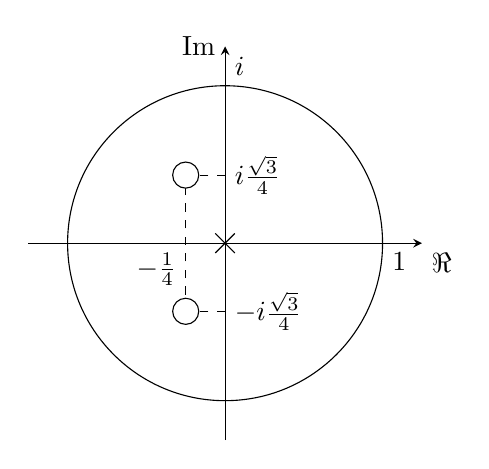
\begin{tikzpicture}[scale=0.5]

		% Axes:
		\draw [-stealth] (-5,0) -- (5,0) node [below right]  {$\Re$};
		\draw [-stealth] (0,-5) -- (0,5) node [left] {$\Im$};

		% pole
		\node[cross out,draw=black] at (0,0) {};

		\draw[dashed] (-1,-1.73) -- (-1,1.73) node[midway, below left]{$-\frac{1}{4}$};
		
		% zeros    
		\draw[dashed] (0,1.73) node[right] {$i \frac{\sqrt{3}}{4}$} --  (-1,1.73) node[solid, fill=white, circle,draw=black] {};
		\draw[dashed] (0,-1.73) node[right] {$-i \frac{\sqrt{3}}{4}$} --  (-1,-1.73) node[solid, fill=white, circle,draw=black] {};

		% unit circle
		\draw (0,0) circle (4);
		\node[below right] at (4,0) {$1$};
		\node[above right] at (0,4) {$i$};
	\end{tikzpicture}
\end{figure}
\FloatBarrier

\begin{defn}
	We say that $W(z)=\frac{C(z)}{A(z)}$ is:
	\begin{itemize}
		\item \textbf{asymptotically stable} if all \emph{poles} are such that $|z|<1$.
		\item \textbf{minimum phase} if all \emph{zeros} are such that $|z|<1$.
	\end{itemize}
\end{defn}

\begin{thm}
	Consider a rational transfer function $W(z)$ fed by a \gls{sp} $v(t)$, $y(t)=W(z)v(t)$. If
	\begin{itemize}
		\item $v(t)$ is a \gls{ssp};
		\item $W(z)$ is asymptotically stable;
	\end{itemize}
	then $y(t)$ is well-defined and is also \emph{stationary} (is a \gls{ssp}).
\end{thm}

In the case of ARMA processes, the input is a \gls{wn}, which is stationary by definition. Thus we just need to check the asymptotical stability.

In general one can factorize the denominator:
\begin{align*}
	y(t)&=\frac{C(z)}{A(z)}v(t)=\frac{C(z)}{(z-p_{1})(z-p_{2})\cdots(z-p_{m})}v(t)\\
	&=C(z)\cdot\frac{1}{z-p_{1}}\cdot\frac{1}{z-p_{2}}\cdots\frac{1}{z-p_{m}}v(t)\\
	&=\frac{1}{z-p_{m}}\left[ \frac{1}{z-p_{m-1}}\left[ \cdots\frac{1}{z-p_{1}}\left[ C(z)v(t) \right]   \right]   \right]  
\end{align*}

\begin{figure}[htpb]
	\centering
	\begin{tikzpicture}

	% place nodes
	\node [block] (c) at (0,0) {$C(z)$};
	\node [block] (p1) at (2.5,0) {$\frac{1}{z-p_1}$};
	\node [block] (p2) at (5,0) {$\frac{1}{z-p_2}$};

	\node [block] (pm) at (7.5,0) {$\frac{1}{z-p_m}$};

	% connect nodes
	\draw[stealth-] (c) -- ++(-1.5,0) node[midway,above] {$v(t)$};

	\draw[-stealth]  (c.east) -- (p1.west) node[midway,above] {$x_1(t)$};
	\draw[-stealth] (p1.east) -- (p2.west) node[midway,above] {$x_2(t)$};

	\draw[-] (p2.east) -- ++(0.2,0) node[at end,right] {$\ldots$};
	\draw[stealth-] (pm.west) -- ++(-0.4,0);
	\draw[-stealth] (pm.east) -- ++(1,0) node[midway,above] {$y(t)$};

	\end{tikzpicture}
\end{figure}
\FloatBarrier
%!TEX root = ../main.tex
Now, let us consider the \gls{sp} $y(t)$ obtained as output of an asymptotically stable digital filter $F(z)$ fed by a \gls{ssp} $v(t)$ as input, but with a generic initialization (not steady-state output).

\begin{figure}[htpb]
	\centering
	\begin{tikzpicture}
		% place nodes
		\node [block] (f) at (0,0) {$F(z)$};

		% connect nodes
		\draw [stealth-] (f.west) -- ++(-2,0) node[midway,above] {$v(t)$};
		\draw [-stealth] (f.east) -- ++(2,0)  node[midway,above] {$y(t)$};
	\end{tikzpicture}
\end{figure}
\FloatBarrier

\begin{thm}
	There is just one stationary output which corresponds to the steady-state solution. However, if $F(z)$ is asymptotically stable, then all possible outputs obtained for different initialization of the digital filter $F(z)$ tends asymptotically (as $t \rightarrow \infty$) to the steady-state solution, i.e. to the stationary output.
\end{thm}

\fg{0.7}{steady-state}

\section{Weak (wide-sense) characterization of AR, ARMA processes}
Our goal now is to consider AR and ARMA processes and compute their mean $m_y$ and covariance function $\gamma_y(\tau)$.

%Since the steady-state solution is an MA($\infty$) process we could use such results but are too diffucult

We'll rely on the recursive equation characterizing such processes.

\subsection{AR processes}

Let us consider the AR($1$) (or equivalently ARMA($1,0$)) process generated according to:
\begin{align*}
	y(t)=a \cdot y(t-1)+e(t) \quad \text{where} \quad e(t) \sim \WN(0, \lambda^{2})
\end{align*}

Operatorial representation for $y(t)$:

\begin{align*}
	y(t)&=z^{-1} a y(t)+e(t) \\
	\left(1-z^{-1} a\right) y(t)&=e(t) \\
	y(t)&=\frac{1}{1-z^{-1} a} e(t)
\end{align*}

The transfer function with positive powers (to identify zeros and poles) is $y(t)=\frac{z}{z-a} e(t) \quad$.

There is just one pole: $z=a .$

The process generating system is asymptotically stable if $|a| <1$. 

Since $e(t)$ is a \gls{ssp} (by definition of \gls{wn}), when $|a| <1$ the steady-state output process $y(t)$ is a \gls{ssp}.

\textbf{Mean.}
Start from the time-domain representation and apply expectation to both sides:
\[
	\E[y(t)]=\E[a \cdot y(t-1)+e(t)] \implies \E[y(t)]=a \cdot \E[y(t-1)]+\E[e(t)]
\]
Thanks to stationarity $\E[y(t)]=\E[y(t-1)]=m_{y}$, so that $m_{y}=a \cdot m_{y}+m_{e}$.
Then:
$$
m_{e}=0 \implies  m_{y}=0
$$
\textbf{Variance.}
Let us compute
\[
	\gamma_{y}(0)=\E\left[\left(y(t)-m_{y}\right)^{2}\right]
\]
Remember that $m_{y}=0$. Start from $y(t)=a \cdot y(t-1)+e(t)$, take the square and apply operator $\E[\cdot]$ to both side:
\begin{align*}
	\gamma_{y}(0)&=\E\left[(y(t))^{2}\right]\\
	&=\E\left[(a \cdot y(t-1)+e(t))^{2}\right]\\
	&=a^{2} \E\left[y(t-1)^{2}\right]+\E\left[e(t)^{2}\right]+2 a \E[y(t-1) e(t)]\\
\end{align*}
Mid-term evaluation:
\[
	2 a \E[y(t-1) e(t)]=0,
\]
indeed, by using the MA($\infty$) representation for $y(t-1)$ (AR process):
$$
y(t-1)=e(t-1)+a \cdot e(t-2)+a^{2} \cdot e(t-3)+a^{3} \cdot e(t-4)+\cdots
$$
we have that:
\[
	\E[e(t) y(t-1)]=\E\left[e(t) \cdot\left(e(t-1)+a \cdot e(t-2)+a^{2} \cdot e(t-3)+a^{3} \cdot e(t-4)+\cdots\right)\right]=0
\]
(all products give null contribution thanks to the whiteness property).


$\E\left[(y(t-1))^{2}\right]=\gamma_{y}(0)$

$\E\left[(e(t))^{2}\right]=\lambda^{2}$

Hence,
\[
	\gamma_{y}(0)=a^{2} \gamma_{y}(0)+\lambda^{2} \implies \gamma_{y}(0)=\frac{\lambda^{2}}{1-a^{2}}
\]
\textbf{Covariance.}
Remember that $m_{y}=0$ and substitute $y(t)=a \cdot y(t-1)+e(t)$,
\begin{align*}
	\gamma_{y}(1)&=\E\left[\left(y(t)-m_{y}\right) \cdot\left(y(t-1)-m_{y}\right)\right]\\
	&=\E[y(t) y(t-1)]\\
	&=\E[(a \cdot y(t-1)+e(t))y(t-1)]\\
	&=a \cdot \E\left[(y(t-1))^{2}\right]+\E[e(t) y(t-1)]
\end{align*}

We already know that $\E\left[(y(t-1))^{2}\right]=\gamma_{y}(0)$, while as before $\E[e(t) y(t-1)]=0$.
$$
\gamma_{y}(1)=a \cdot \gamma_{y}(0)=a \cdot \frac{\lambda^{2}}{1-a^{2}}
$$
Arguing the same way,
\[
	\gamma_{y}(2)=a \cdot \gamma_{y}(1)=a^{2} \cdot \frac{\lambda^{2}}{1-a^{2}}
\]
Summary:
\begin{equation*}
	\boxed{
		\begin{cases}
			\gamma_{y}(0)=\frac{\lambda^{2}}{1-a^{2}} \\
			\gamma_{y}(1)=\gamma_{y}(-1)=a \cdot \gamma_{y}(0) \\
			\gamma_{y}(2)=\gamma_{y}(-2)=a \cdot \gamma_{y}(1) \\
			\quad\vdots
		\end{cases}
	}
\end{equation*}

Recursive expression for $\gamma_{y}(\tau)$
$$
	\gamma_{y}(\tau)=a^{|\tau|}\cdot \frac{\lambda^{2}}{1-a^{2}}
$$
This result has been established for a generic AR($1$) process.
Those equations are called \emph{Yule--Walker equations} for AR($1$) process.

\begin{figure}[htpb]
	\centering
	\begin{subfigure}{.5\textwidth}
		\centering
		\scalebox{0.7}{
		\begin{tikzpicture}

			\begin{axis}
			[
				axis x line=middle,
			    axis y line=middle,
			    ytick = \empty,
				xlabel={$\tau$},
				ylabel={$\gamma_y(\tau)$},
				xmin=-6, xmax=6,
				ymin=-1, ymax=1.5,
			]
			\addplot+[domain=-6:6, samples at={-6,...,6},color=black,mark options={fill=black}]{(0.5)^abs(x)/(1-(-0.5)^2)};
			\end{axis}

		\end{tikzpicture}}
		\caption{Case $0<a<1$.}
	\end{subfigure}%
	\begin{subfigure}{.5\textwidth}
		\centering
		\scalebox{0.7}{
		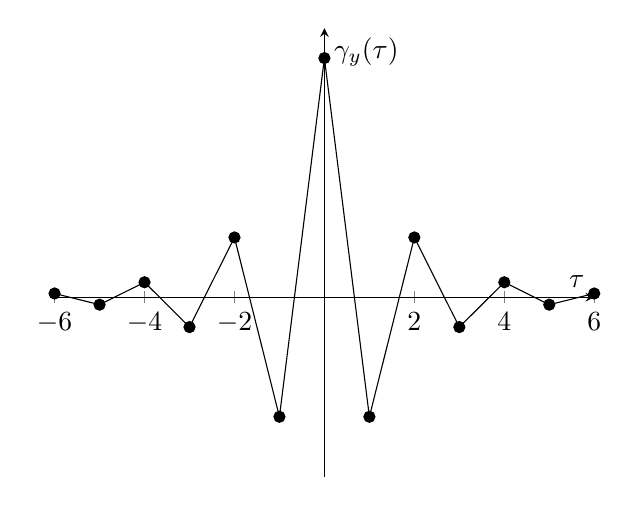
\begin{tikzpicture}

		\begin{axis}
		[
			axis x line=middle,
			axis y line=middle,
			ytick = \empty,
			xlabel={$\tau$},
			ylabel={$\gamma_y(\tau)$},
			xmin=-6, xmax=6,
			ymin=-1, ymax=1.5,
		]
		\addplot+[domain=-6:6, samples at={-6,...,6},color=black,mark options={
		fill=black}]{(-0.5)^abs(x)/(1-(-0.5)^2)};
		\end{axis}

		\end{tikzpicture}}
		\caption{Case $-1<a<0$.}
	\end{subfigure}
	\caption{Graphical representation of the covariance function for AR($1$) processes.}
\end{figure}
\FloatBarrier

\subsection{ARMA processes}
Let us consider the ARMA($m,n$) process generated according to:
\begin{align*}
	y(t) & = a_{1} y(t-1)+\cdots+a_{m} y(t-m)\\
	     &\quad +c_{0} e(t)+\cdots+c_{n} e(t-n) \quad \text{where} \quad e(t) \sim \WN(0, \lambda^{2})
\end{align*}


\textbf{Mean.}
\begin{align*}
	\E[y(t)] &=\E\left[a_{1} y(t-1)+\cdots+a_{m} y(t-m)+c_{0} e(t)+\cdots+c_{n} e(t-n)\right] \\
	&=a_{1} \E[y(t-1)]+\cdots+a_{m} \E[y(t-m)]+c_{0} \E[e(t)]+\cdots+c_{n} \E[e(t-n)]
\end{align*}
$$
m_{y}=a_{1} m_{y}+\cdots+a_{m} m_{y}+c_{0} \cdot 0+\cdots+c_{n} \cdot 0
$$

By asymptotic stability we can prove\footnote{It will not be done in this text.} that $(1-a_1-\cdots-a_m)\neq 0$, i.e. $m_{y}=0$.

\textbf{Covariance.}
\begin{align*}
	\gamma_{y}(0) = \E[y(t)^{2}] &= \E\left[\left(a_{1} y(t-1) + \cdots + a_{m} y(t-m) + c_{0} e(t) + \cdots + c_{n} e(t-n)\right)^{2}\right]\\
	&= a_{1}^{2} \E[y(t-1)^{2}] + a_{2}^{2} \E[y(t-2)^{2}] + \cdots+a_{m}^{2} \E[y(t-m)^{2}]\\
	&\qquad + 2 a_{1} a_{2} \E[y(t-1) y(t-2)] + 2 a_{1} a_{3} \E[y(t-1) y(t-3)] + \cdots \\
	&\qquad + c_{0}^{2} \E[e(t)^{2}] + c_{1}^2 \E[e(t-1)^2] + \cdots+c_{n}^2 \E[e(t-n)^2]\\
	&\qquad + 2 a_{1} c_{0} \E[y(t-1) e(t)] + 2 a_{1} c_{1} \E[y(t-1) e(t-1)] + \cdots\\
	&= (a_{1}^{2} + a_{2}^{2} + \cdots+a_{m}^{2})\cdot\gamma_{y}(0)\\
	&\qquad + 2 a_{1} a_{2} \gamma_{y}(1) + 2 a_{1} a_{3} \gamma_{y}(2) + \cdots \\
	&\qquad + (c_{0}^{2} + c_{1}^2 + \cdots+c_{n}^2)\cdot\lambda^2\\
	&\qquad + 2 a_{1} c_{0} \E[y(t-1) e(t)] + 2 a_{1} c_{1} \E[y(t-1) e(t-1)] + \cdots\\
\end{align*}

Then
\[
	\gamma (1)=\E[y(t) y(t-1)] = \E\left[\left(a_{1} y(t-1)+\cdots+a_{m} y(t-m)+c_{0} e(t)+\cdots+c_{n} e(t-n)\right) y(t-1)\right]
\]
Proceeding this way we get $m$ variables and $m$ linear equations (\emph{Yule--Walker equations} for an ARMA process).

Then $\gamma_{y}(m), \gamma_{y}(m+1), \ldots$ can be recursively computed from $\gamma_{y}(0), \gamma_{y}(1), \ldots, \gamma_{y}(m-1)$.
\input{lectures/2022_03_03}
\input{lectures/2022_03_07}
%!TEX root = ../main.tex
\section{Non-zero mean ARMA processes}\label{sec:non-zero-mean-arma}
Consider now $y(t)$ ARMA process generated as the steady-state output of a linear operator $W(z)$ that receive as input $e(t)$, where $e(t) \sim \WN(\mu, \lambda^{2})$, with $\mu\neq0$.

\begin{thm}[Gain theorem]\label{thm:gain-theorem}
	The steady-state output is constant and it holds that:
	\[
		\E[y(t)]=m_{y}=W(z)\big|_{z=1} \cdot \mu
	\]
\end{thm}

Indeed:
\begin{align*}
		\E[y(t)] &=\E\left[a_{1} y(t-1)+\cdots+a_{m} y(t-m)+c_{0} e(t)+\cdots+c_{n} e(t-n)\right] \\
		&=a_{1} \E[y(t-1)]+\cdots+a_{m} \E[y(t-m)]+c_{0} \E[e(t)]+\cdots+c_{n} \E[e(t-n)]
\end{align*}
$$
m_{y}=a_{1} m_{y}+\cdots+a_{m} m_{y}+c_{0} \cdot \mu+\cdots+c_{n} \cdot \mu
$$
i.e.
\[
	m_{y}=\frac{c_{0}+c_{1}+\cdots+c_{n}}{1-a_{1}-\cdots-a_{m}} \cdot \mu=W(1) \cdot \mu.
\]
For any $t$, we define two new \textbf{unbiased processes}:
$$
\boxed{
	\begin{cases}
		\tilde{y}(t)=y(t)-m_{y}\\
		\tilde{e}(t)=e(t)-m_{e}
	\end{cases}
}
$$
such that their mean is zero. Moreover we have that:
\begin{align*}
	\tilde{y}(t)&= y(t)-m_{y}\\
	&= a_{1} y(t-1)+\cdots+a_{m} y(t-m)+c_{0} e(t)+\cdots+c_{n} e(t-n)-m_{y} \\
	&= a_{1}\left(\tilde{y}(t-1)+m_{y}\right)+\cdots+a_{m }\left(\tilde{y}(t-m)+m_{y}\right)+\\
	&\qquad +c_{0}\left(\tilde{e}(t)+m_{e}\right)+\cdots+c_{n}\left(\tilde{e}(t-n)+m_{e}\right)-m_{y} \\
	&= a_{1} \tilde{y}(t-1)+\cdots+a_{m} \tilde{y}(t-m)+c_{0} \tilde{e}(t)+\cdots+c_{n} \tilde{e}(t-n) \\
	&\qquad \underbrace{-\left(1-a_{1}-\cdots-a_{m}\right) m_{y}+\left(c_{0}+\cdots + c_{n}\right) m_{e}}_{=0\text { since } m_{y}=\frac{c_{0}+c_{1}+\cdots+c_{n}}{1-a_{1}-\cdots-a_{m }} m_{e}=W(1) \cdot \mu} \\
	&=a_{1} \tilde{y}(t-1)+\cdots+a_{m} \tilde{y}(t-m)+c_{0} \tilde{e}(t)+\cdots+c_{n} \tilde{e}(t-n)
\end{align*}
where $\tilde{e}(t)\sim \WN(0, \lambda^{2})$, hence this is a standard zero mean ARMA process. $\tilde{y}(t)$ is the steady-state solution to $W(z)=\frac{A(z)}{C(z)}$ \emph{with the same transfer function} fed by $\tilde{e}(t)$.
\[
	\boxed{y(t)=W(z)e(t) \iff \tilde{y}(t)=W(z)\tilde{e}(t)}
\]

In addition, the \emph{covariance function is also the same}:
$$
	\boxed{\gamma_{y}(\tau)=\E\left[\left(y(t)-m_{y}\right) \cdot\left(y(t-\tau)-m_{y}\right)\right]=\E[(\tilde{y}(t)) \cdot(\tilde{y}(t-\tau))]=\gamma_{\tilde{y}}(\tau)}
$$

We can see this method graphically. Thanks to linearity, this picture:

\begin{figure}[htpb]
	\centering
	\begin{tikzpicture}
		% place nodes
		\node [sum] (sum) at (0,0){};
		\node [block,right=2cm of sum] (w) {$W(z)$};

		% connect nodes
		\draw[stealth-] (sum.north) -- ++(0, 1)
			node[midway, left]{$\mu$}
			node[very near start, right] {$+$};

		\draw[stealth-] (sum.south) -- ++(0,-1)
			node[midway, left]{$\tilde e(t)$}
			node[very near start, right] {$+$};

		\draw[-stealth] (sum.east) -- (w.west) node[midway, above] {$e(t)$};
		\draw[-stealth] (w.east) -- ++(2,0) node[midway, above] {$y(t)$};
	\end{tikzpicture}
\end{figure}
\FloatBarrier
is equivalent to the following:
\begin{figure}[htpb]
	\centering
	\begin{tikzpicture}
		% place nodes
		\node [sum] (sum) at (0,0){};
		\node [block,above left=0.5cm and 2cm of sum] (wm) {$W(z)$};
		\node [block,below left=0.5cm and 2cm of sum] (we) {$W(z)$};

		% connect nodes
		\draw[stealth-] (wm.west) -- ++(-2,0) node[midway, above]{$\mu$};
		\draw[stealth-] (we.west) -- ++(-2,0) node[midway, above]{$\tilde e(t)$};

		\draw[-stealth] (wm.east) -| (sum.north)
			node[near start,above] {$m_y$}
			node[very near end, right] {$+$};
		\draw[-stealth] (we.east) -| (sum.south)
			node[near start,above] {$\tilde y(t)$}
			node[very near end, right] {$+$};

		\draw[-stealth] (sum.east) -- ++(2,0) node[midway, above] {$y(t)$};
	\end{tikzpicture}
\end{figure}
\FloatBarrier

\section{ARMAX (and ARX) processes}

\begin{defn}
	Let $e(t) \sim \WN(0, \lambda^{2})$. An \textbf{ARMAX process} of order $m,n,p,d$ is a process generated by a \gls{wn} $e(t)$ and by an \textbf{eXogenous} deterministic input $u(t)$, according to:
	\begin{equation*}
	   \boxed{
		   \begin{aligned}
				y(t)&=a_{1} y(t-1)+a_{2} y(t-2)+\cdots+a_{m} y(t-m) &\text{AR($m$) part}\\
				&\qquad+c_{0} e(t)+c_{1} e(t-1)+\cdots+c_{n} e(t-n) &\text{MA($n$) part} \\
				&\qquad+b_{0} u(t-d)+b_{1} u(t-d-1)+\cdots+b_{p} u(t-d-p)  &\text{X($d,p$) part}
			\end{aligned}
		}
	\end{equation*}
\end{defn}

ARMAX($m,n,p,d$) denotes an ARMAX process of orders $m,n,p$ with delay between the input $u(t)$ and output $y(t)$ equal to $d$.

ARX($m,p,d$) equals to ARMAX($m,0,p,d$).

Then:
\begin{gather*}
	y(t) = \frac{(b_{0}+b_{1} z^{-1}+\cdots+b_{p} z^{-p}) z^{-d}}{(1-a_{1} z^{-1}-a_{2} z^{-2}-\cdots-a_{m} z^{-m})} u(t)
	+ \frac{(c_{0}+c_{1} z^{-1}+\cdots+c_{n} z^{-n})}{(1-a_{1} z^{-1}-a_{2} z^{-2}-\cdots-a_{m} z^{-m})} e(t) \\
	\boxed{
		y(t) =
		\underbrace{\frac{B(z) z^{-d}}{A(z)} u(t)}_{\text{deterministic}}
		+\underbrace{\frac{C(z)}{A(z)} e(t)}_{\substack{\text{stochastic}\\ \text{(ARMA)}}}
	}
\end{gather*}
where:
\begin{gather*}
	\boxed{B(z) = \left(b_{0}+b_{1} z^{-1}+\cdots+b_{p} z^{-p}\right)}\\
	\boxed{C(z) = \left(c_{0}+c_{1} z^{-1}+\cdots+c_{n} z^{-n}\right)}\\
	\boxed{A(z) = \left(1-a_{1} z^{-1}-a_{2} z^{-2}-\cdots-a_{m} z^{-m}\right)}
\end{gather*}

Both $\frac{B(z) z^{-d}}{A(z)}$ and $\frac{C(z)}{A(z)}$ are transfer functions.

In the ARX process $C(z)=1$.

\chapter{Analysis in the Frequency Domain}
\begin{defn}
	The \textbf{spectral density} or \textbf{spectrum} of a \gls{ssp} $y(t)$ is defined as:
	\[
		\Gamma_{y}(\omega)=\sum_{\tau=-\infty}^{+\infty} \gamma_{y}(\tau) e^{-j \omega \tau} \qquad \omega \in \RR
	\]
\end{defn}

In other words, $\Gamma_y(\omega)=\mathcal{F}\{\gamma_y(\tau)\}$ is defined as the discrete Fourier transform of the covariance function.

\textbf{Properties of $\Gamma_{y}(\omega)$:}
\begin{enumerate}
	\item is a \textbf{real} function of the real variable $\omega$,
	$$
		\Im\left(\Gamma_{y}(\omega)\right)=0 \quad \forall \omega \in \RR
	$$
	\item is a \textbf{positive} function,
	$$
		\Gamma_{y}(\omega) \geq 0 \quad \forall \omega \in \RR
	$$
	\item is an \textbf{even} function,
	$$
		\Gamma_{y}(\omega)=\Gamma_{y}(-\omega) \quad \forall \omega \in \RR
	$$
	\item is \textbf{$2\pi$-periodic}:
	$$
		\Gamma_{y}(\omega)=\Gamma_{y}(\omega+k \cdot 2 \pi) \quad \forall \omega \in \RR, \forall k \in \mathbb{Z}
	$$
\end{enumerate}

\begin{rem}
As a consequence of 3. and 4., we will plot the spectral density in $[0, \pi]$.
\end{rem}

\begin{exa}[Density of a \gls{wn}]
	Let us consider $e(t) \sim \WN(\mu, \lambda^{2})$.

	Covariance function:
	\[
		\gamma_{e}(\tau) =
		\begin{cases}
			\lambda^{2}, & \text { if } \tau=0, \\
			0, & \text { if } \tau \neq 0.
		\end{cases}
	\]
	Spectral density:
	\[
		\Gamma_{e}(\omega) =\sum_{\tau=-\infty}^{+\infty} \gamma_{e}(\tau) e^{-j \omega \tau}=\underbrace{\gamma_{e}(0)}_{=\lambda^2} \underbrace{e^{-j \omega 0}}_{=1}+\underbrace{\gamma_{e}(1)}_{=0} e^{-j \omega} + \underbrace{\gamma_{e}(-1)}_{=0} e^{j \omega}+\cdots = \lambda^{2}
	\]
	\gls{wn} have constant and equal to $\lambda^{2}$ spectral density.
\end{exa}
\newpage
\begin{exa}
Let us consider the generic MA($1$) process defined by $y(t)=e(t)+c \cdot e(t-1)$, with $c \in \RR$, $e(t)\sim \WN(0,1)$.\\
We know that:
\begin{align*}
	&\gamma_{y}(0)=(1^{2}+c^{2})\cdot \lambda^{2}=(1+c^{2})\\
	&\gamma_{y}(1)=(1 \cdot c) \cdot \lambda^{2}=c \\
	&\gamma_{y}(\tau)=0, \text{ otherwise.}
\end{align*}
Spectral density:
\begin{align*}
	\Gamma_{y}(\omega)&=\sum_{\tau=-\infty}^{+\infty} \gamma_{y}(\tau) e^{-j \omega \tau}\\
	&=\gamma_{y}(0)+\gamma_{y}(1)(e^{-j \omega})+\gamma_{y}(-1)(e^{+j \omega}) \\
	&=1+c^{2}+c(e^{-j \omega}+e^{j \omega})
\end{align*}

Remembering Euler's representation of the exponential:
$$
	e^{-j \omega}+e^{j \omega}=\cos (\omega)-j \sin (\omega)+\cos (\omega)+j \sin (\omega)=2 \cos (\omega),
$$
we have:
$$
	\Gamma_y(\omega)=1+c^{2}+2 c \cdot \cos (\omega).
$$
which is real, non-negative, even and $2 \pi$-periodic.
\end{exa}

\begin{thm}[Fundamental theorem of the spectral analysis]
    Let the process $y(t)$ be the steady-state output of an asymptotically stable digital filter fed by an \gls{ssp}, i.e. $y(t)=W(z) v(t)$. Then, the following formula for the spectral density of $y(t)$ holds:
\[
	\boxed{\Gamma_{y}(\omega)=\left|W(e^{j \omega})\right|^{2} \cdot \Gamma_{v}(\omega)}
\]
where $W(e^{j \omega})$ is called \textbf{frequency response} of $W(z)$.
\end{thm}

If the input $v(t)$ is a \gls{wn} with variance $\lambda^{2}$, then:
$$
\Gamma_{y}(\omega)=\left|W(e^{j \omega})\right|^{2} \cdot \lambda^2
$$
In addition, remember that
\[
\left|W\left(e^{j \omega}\right)\right|^{2}=W\left(e^{j \omega}\right)\cdot W\left(e^{-j \omega}\right)
\]

\begin{exa}
    Let us consider again the generic MA($1$) process defined by $y(t)=e(t)+c \cdot e(t-1)$, with $c \in \RR$, $e(t)\sim \WN(0,1)$.
    
    Then
    \[
    y(t)=(1+cz^{-1})e(t)=W(z)e(t)
    \]
    Let compute spectral density in alternative way with the fundamental theorem of the spectral analysis:
\begin{align*}
	\Gamma_{y}(\omega)&=\left|W(e^{j \omega})\right|^{2} \cdot \Gamma_{e}(\omega)\\
	&=W\left(e^{j \omega}\right)\cdot W\left(e^{-j \omega}\right)\cdot 1\\
    &=\left(1+c e^{-j \omega}\right)\left(1+c e^{+j \omega}\right)\\
    &=1+ce^{j\omega}+ce^{-j\omega}+c^2\\
    &=1+c^2+c\left(e^{j\omega}+e^{-j\omega}\right) = 1 + c^2 +2c\cdot \cos{(\omega)}
\end{align*}
\end{exa}

See Figure \ref{fig:example-density} for the plot of the spectral density.

\begin{figure}[htpb]
	\centering
	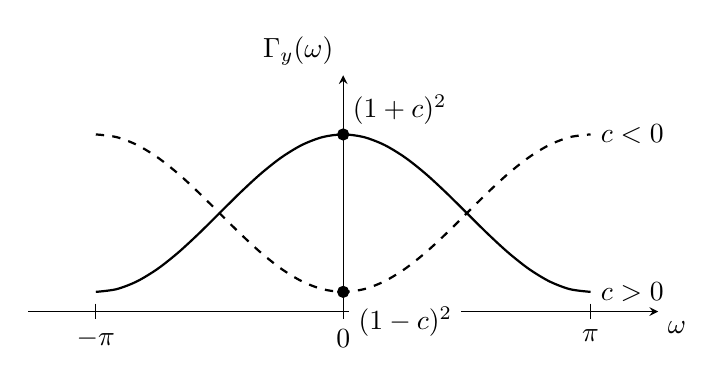
\begin{tikzpicture}
	    
	    %\draw[very thin,color=gray] (-3.14,-1) grid (3.14,3);
	    \draw[-stealth, name path=xax] (-4, 0) -- (4, 0) node (ynode) [below right] {$\omega$};
	    \draw[-stealth, name path=yax] ( 0, 0) -- (0, 3) node (xnode) [above left] {$\Gamma_y(\omega)$};
	    % \x r means to convert ’\x’ from degrees to _r_adians:
	    \draw[name path=cpos, domain=-pi:pi, smooth, variable=\x, black, thick] plot ({\x}, {1+0.5*0.5+2*0.5*cos(\x r)}) node[right]{$c>0$};
	    \draw[name path=cneg, domain=-pi:pi, smooth, variable=\x, black, dashed, thick] plot ({\x}, {1+0.5*0.5-2*0.5*cos(\x r)}) node[right]{$c<0$};
	    
	    \draw[-] (-pi,0.1)--(-pi,-0.1) node[below] {$-\pi$};
	    \draw[-] ( pi,0.1)--( pi,-0.1) node[below] {$ \pi$};
	    \draw[-] ( 0 ,0.1)--( 0, -0.1) node[below] {$ 0  $};
	    
	    \draw [name intersections={of=cpos and yax, by=x}, fill] (x)
	        circle [radius=2pt]
	        node[above right] {$(1+c)^2$};


	    \draw [name intersections={of=cneg and yax, by=x}, fill] (x)
	        node[fill=white,below right,xshift=2pt,yshift=-2pt] {$(1-c)^2$}
	        circle [radius=2pt];

	\end{tikzpicture}
	\caption{Spectral density for MA($1$) process.}
	\label{fig:example-density}
\end{figure}
%!TEX root = ../main.tex
\section{Spectrum of a \glsentrylong{ssp}}
Given $y(t)$ a \gls{ssp}, we can compute:
\begin{itemize}
	\item Fourier transform
	\[
		\Gamma _{y}(\omega)=\fou{\gamma _{y}(\tau )}=\sum_{\tau =-\infty }^{+\infty} \gamma _{y}(\tau ) e^{-j\omega \tau } \qquad \omega \in [0,\pi ]
	\]
	\item Anti-Fourier transform
	\[
		\gamma _{y}(\tau)=\ifou{\Gamma _{y}(\omega)}=\frac{1}{2\pi }\int_{-\pi }^{\pi } \Gamma _{y}(\omega )e^{j\omega \tau }d\omega  
	\]
\end{itemize}

\begin{rem}
If $\tau =0$ we have
\[
	\gamma _{y}(0)=\E[(y(t)-m_{y})^2 ]=\frac{1}{2\pi }\int_{-\pi }^{\pi } \Gamma _{y}(\omega )d\omega 
\]
\end{rem}
\textbf{Remark.}
There is bijective relationship between the spectrum and the covariance function. Namely to describe $y(t)$ one could use $m_{y}$ and $\gamma _{y}(\tau )$ or $m_{y}$ and $\Gamma _{y}(\omega)$. It gives the same information from a different perspective, but it's useful to understand some properties.

\subsection{An alternative interpretation of the spectral density}
Suppose that an \gls{ssp} $y(t)$ is filtered through an (ideal) pass-band filter:
\fg{0.7}{kinchine-wiener}
where $\tilde{y}(t)$ is the filtered output process.
\begin{thm}[Kinchine--Wiener]
	The spectral density at a fixed $\omega$ equals to the mean energy of process realizations frequency by frequency:
	\[
		\Gamma _{y}(\overline{\omega})=\lim_{\delta  \to 0} \gamma _{\tilde{y}}(0)
	\]
\end{thm}

\begin{exa}
The \gls{wn} spectral density is constant, i.e. \gls{wn} energy is \emph{equally-distributed} all over the frequency domain.
\end{exa}

\begin{figure}[htpb]
	\centering
	\begin{tikzpicture}

	    % x axis
	    \draw[-stealth]
	        (-4,0) -- (0,0) node[below] {$0$}
	        ( 0,0) -- (4,0) node[right] {$\omega$};
	    
	    \draw[-stealth] (0,0) -- (0,2) node[left] {$\Gamma_y(\omega)$};
	    
	    % plot
	    \draw[very thick]
	        (-pi,1) -- (0,1) node[below left] {$\lambda^2$}
	        (  0,1) -- (pi,1){};
	    
	    % projections
	    \draw[dashed]
	        (-pi,1) -- (-pi,0) node[below] {$-\pi$}
	        ( pi,1) -- ( pi,0) node[below] {$ \pi$}
	        {};

	\end{tikzpicture}
\end{figure}
\FloatBarrier

\begin{exa}
Consider the AR($1$) process $y(t)=ay(t-1)+e(t)$.
\begin{itemize}
	\item if $a>0$ the sign tends to be maintained;
	\item if $a<0$ the sign tends to change.
\end{itemize}
The transfer function is $y(t)=\frac{1}{1-az^{-1} }e(t)$, then
\begin{align*}
	\Gamma _{y}(\omega )&=\left|\frac{1}{1-ae^{-j\omega } }\right|^2 \cdot\underbrace{\Gamma _{e}(\omega )}_{=\lambda^2 } = \frac{1}{1-ae^{-j\omega}}\cdot\frac{1}{1-ae^{j\omega}} \cdot\lambda^2\\
	&=\frac{1}{1+a^2 e^{-j\omega }\cdot e^{j\omega }-ae^{-j\omega}-ae^{j\omega}} \cdot \lambda^2\\
	&=\frac{1}{1+a^2 -a\left( \frac{e^{j\omega}+e^{-j\omega}}{2} \right)\cdot 2}\\
	&=\frac{1}{1+a^2-2a\cos (\omega)} \cdot\lambda^2
\end{align*}
\end{exa}
Depending on the values of $a$ we have different behaviors.

If $a>0$ energy is concentrated at low frequencies
\fg[Left: signal. Right: spectrum.]{0.8}{ar-1-frequency-fig1}
If $a<0$ energy is concentrated at larger frequencies
\fg[Left: signal. Right: spectrum.]{0.8}{ar-1-frequency-fig2}

\begin{exa}
Consider the ARMA process $y(t)=\frac{C(z)}{A(z)}e(t)$
\[
	\Gamma _{y}(\omega )=\left|\frac{C(e^{j\omega})}{A(e^{j\omega})}\right|^2 \cdot\lambda^2 =\frac{C(e^{j\omega})}{A(e^{j\omega} )} \cdot \frac{C(e^{-j\omega})}{A(e^{-j\omega} )}\cdot\lambda^2 
\]
$y(t)$ has a \emph{rational} spectral density. The reverse is also true:
\[
	y(t) \text{ ARMA} \iff W(z) \text{ rational}
\]
\end{exa}
Indeed we have the following result:
\begin{thm}
	Let $y(t)$ be a \gls{ssp} with rational spectral density.
	Then, there exists a \gls{wn} process $\xi(t)$ with suitable mean and variance and a rational transfer function $W(z)$ such that:
	\[
		y(t)=W(z)\xi(t)
	\]
	i.e. $y(t)$ is an ARMA process.
\end{thm}

However, the \emph{choice} of $\xi(t)$ and of $W(z))$ \emph{is not unique}.
The \emph{same} process $y(t)$ can be generated according to an infinite number of different ARMA models.

Let $y(t)=W(z)\xi(t)$, where $\xi(t)$ is a $\WN\sim(\mu,\lambda^2)$. Our goal is show how to construct $\tilde{W}(z)$ and $\tilde{\xi}(t)$ such that $\tilde{W}(z)\neq W(z)$ and $\tilde{\xi}(t)\neq \xi(t)$, but $y(t)=\tilde W(z)\tilde\xi(t)$. Let us consider four different cases:
\begin{enumerate}
	\item 
	Let $\alpha \in \RR$
	\[
		y(t)=W(z) \xi(t) = \underbrace{\frac{W(z)}{\alpha}}_{\tilde{W}(z)} \cdot \underbrace{\alpha \xi(t)}_{\tilde{\xi}(t)} = \tilde{W}(z)\tilde{\xi}(t)
	\]
	where they are still both respectively a rational transfer function and a \gls{wn}, indeed:
	\begin{align*}
		\E[\tilde{\xi}(t)]&=\E[\alpha \xi(t)]=\alpha \E[\xi(t)]=\alpha \mu\\
		\gamma_{\tilde{\xi}}(\tau)&=\E[(\alpha\xi(t)-\alpha\mu)(\alpha \xi(t-\tau)-\alpha \mu)]=\alpha^2 \E[(\xi(t)-\mu)( \xi(t-\tau)- \mu)] = \alpha^2 \gamma_{\xi}(\tau)
	\end{align*}

	\item 
	Let $n \in \NN$
	\[
		y(t)=W(z) \xi(t)=W(z) \cdot \frac{z^{n}}{z^{n}} \xi(t)=\left[z^{n} \cdot W(z)\right] \xi(t-n)=\tilde{W}(z) \tilde{\xi}(t)
	\]
	where they are still both respectively a rational transfer function and a \gls{wn}, indeed:
	\begin{align*}
		\E[\tilde{\xi}(t)]&=\E[\xi(t-n)]=\mu \\
		\gamma_{\tilde{\xi}}(\tau)&=\E[(\xi(t-n)-\mu)(\xi(t-n-\tau)-\mu)]=\gamma_{\xi}(\tau)
	\end{align*}

	\item 
	Let $p \in \CC$ such that $|p|<1$
	\[
		y(t)=W(z) \xi(t) = \underbrace{\left[W(z) \cdot \frac{z-p}{z-p}\right]}_{\tilde{W}(z)} \xi(t)=\tilde{W}(z) \xi(t)
	\]
	where they are still both respectively a rational transfer function and a \gls{wn}.

	\item 
	Let $q$ be a zero of $W(z)$ such that $|q|>1$, that is
	\[
		W(z)=W_{1}(z)\cdot(z-q)
	\]
	then
	\begin{align*}
		y(t)&=W(z) \xi(t)=W_{1}(z) \cdot(z-q) \xi(t)=W_{1}(z) \cdot(z-q) \left[ \frac{z-\frac{1}{q}}{z-\frac{1}{q}}\right] \xi(t)= \\
		&=\underbrace{W_{1}(z)\left(z-\frac{1}{q}\right)}_{\tilde{W}(z)}\cdot\underbrace{\frac{z-q}{z-\frac{1}{q}} \xi(t)}_{\tilde{\xi}(t)} = \tilde{W}(z) \tilde{\xi}(t)
	\end{align*}
	Notice that $\tilde{\xi}$ is well-defined and stationary since we multiplied $\xi(t)$ by an asymptotically stable transfer function ($|z|=\left|\frac{1}{q}\right|<1$).\\
	Moreover they are still both respectively a rational transfer function and a \gls{wn}, indeed let us compute the spectral density of $\tilde{\xi}(t)$:
	\begin{align*}
		\Gamma_{\tilde\xi}(\omega) &=\frac{\left|e^{j \omega}-q\right|^{2}}{\left|e^{j \omega}-\frac{1}{q}\right|^{2}} \cdot \lambda^{2}=\frac{\left(e^{j \omega}-q\right)\left(e^{-j \omega}-q\right)}{\left(e^{j \omega}-\frac{1}{q}\right)\left(e^{-j \omega}-\frac{1}{q}\right)} \cdot \lambda^{2}\\
		&=\frac{1+q^{2}-q\left(e^{j \omega}+e^{-j \omega}\right)}{1+\frac{1}{q^{2}}-\frac{1}{q}\left(e^{j \omega}+e^{-j \omega}\right)} \cdot \lambda^{2}=\frac{1+q^{2}-2 q \cos (\omega)}{1+\frac{1}{q^{2}}-\frac{2}{q} \cos (\omega)} \cdot \lambda^{2}\\
		&=q^{2} \frac{\frac{1}{q^{2}}+1-\frac{2}{q} \cos (\omega)}{1+\frac{1}{q^{2}}-\frac{2}{q} \cos (\omega)} \cdot \lambda^{2}=q^{2} \cdot \lambda^{2}
	\end{align*}
	which is always constant and characterises a \gls{wn}; while
	\[
		\boxed{\tilde \xi(t) = \frac{z-q}{z-\frac{1}{q}} \xi(t)} \implies \tilde \xi(t+1)-\frac{1}{q}\tilde \xi(t)=\xi(t+1)-q\xi(t)
	\]
	taking $\E[\cdot]$ on both sides
	\[
		m_{\tilde\xi} - \frac{1}{q} m_{\tilde\xi} = \mu - q\mu \implies m_{\tilde\xi} = \frac{1-q}{1-\frac{1}{q}} \cdot \mu = -q \frac{\cancel{1-\frac{1}{q}}}{\cancel{1-\frac{1}{q}}}=  - q \cdot \mu
	\]
	so in the end we have $\boxed{\tilde\xi(t)\sim \WN(-q\mu,q^2 \lambda^2 )}$.

	The quantity
	\[
		\boxed{\frac{z-q}{z-\frac{1}{q}}}
	\]
	is known as \textbf{all-pass filter}.
\end{enumerate}
%!TEX root = ../main.tex

\begin{thm}[Spectral Factorization]
	Let $y(t)$ be a \gls{ssp} with rational spectral density. 
	Then, there exists an unique \gls{wn} process $\xi(t)$ with suitable mean and variance and an unique rational transfer function $W(z)$ such that:
	\begin{align*}
		y(t) = W(z)\xi(t)=\frac{C(z)}{A(z)}\xi(t)
	\end{align*}
    and:
    \begin{enumerate}
		\item $C(z)$ and $A(z)$ are monic (i.e. the coefficients of the maximum degree terms of $C(z)$ and $A(z)$ are equal to 1);
		\item $C(z)$ and $A(z)$ have null relative degree;
		\item $C(z)$ and $A(z)$ are coprime (i.e. they have no common factors);
		\item[4a.]the poles of $W(z)$ are such that $|z|< 1$;
		\item[4b.]the zeros of $W(z)$ are such that $|z|\leq 1$.
    \end{enumerate}
\end{thm}

When all the four conditions above are satisfied, we will say that $y(t) = W(z)\xi(t)$ is a \textbf{canonical representation} of $y(t)$.

\begin{rem}
Conditions 1, 2, and 3 remove any ambiguity due to the process described in Case 1, Case 2, and Case 3, respectively. 

Condition 4a ensures that $W(z)$ is asymptotically stable so that $y(t)$ is well defined, while 4b removes any ambiguity due to the process described in Case 4.
\end{rem}
\begin{exa}
We want to find the canonical representation of:
\begin{align*}
	y(t)=\frac{2+5z^{-1}+2z^{-2}}{z^2+\frac{5}{6}z+\frac{1}{6}}\cdot e(t)  \qquad e(t)\sim \WN(0,1)
\end{align*}
We first need to have the same degree and positive powers, which we can achieved by multiplying by a proper factor and consider a new \gls{wn}:
\begin{equation*}
	y(t)=
	\frac{2+5z^{-1}+2z^{-2}}{z^2+\frac{5}{6}z+\frac{1}{6}}\cdot e(t)
	=\frac{2+5z^{-1}+2z^{-2}}{z^2+\frac{5}{6}z+\frac{1}{6}}\cdot\frac{z^2}{2}\cdot\underbrace{\frac{2}{z^2}\cdot e(t)}_{\eta(t)}
	=\frac{z^2+\frac{5}{2}z+1}{z^2+\frac{5}{6}z+\frac{1}{6}}\cdot \eta(t)
\end{equation*}
where $\eta(t)=2z^{-2}e(t)=2e(t-2)\sim \WN(2\cdot0,4\cdot 1)\sim \WN(0,4)$.\\
We know check if some terms cancel out:
\begin{align*}
	&\text{zeros:}\quad z^2+\frac{5}{2}z+1=(z+2)\left( z+\frac{1}{2} \right)   \implies z_{1,2}=-2,-\frac{1}{2}\\
	&\text{poles:}\quad z^2+\frac{5}{6}z+\frac{1}{6}=\left( z+\frac{1}{3} \right)  \left( z+\frac{1}{2} \right) \implies p_{1,2}=-\frac{1}{3},-\frac{1}{2}
\end{align*}
Then:
\begin{align*}
	y(t)=\frac{(z+2)\cancel{(z+\frac{1}{2})}}{(z+\frac{1}{3})\cancel{(z+\frac{1}{2})}}\cdot \eta(t) 
\end{align*}
We can now make sure that all zeros and poles are strictly inside the unit circle. In this case it is particularly useful to remember the all-pass filter:
\begin{align*}
	y(t)=\frac{z+2}{z+\frac{1}{3}}\cdot\frac{z+\frac{1}{2} }{z+\frac{1}{2}}\cdot\eta(t)=\frac{z+\frac{1}{2}}{z+\frac{1}{3}}\underbrace{\frac{z+2}{(z+\frac{1}{2})}\eta(t)}_{\xi(t)}=\frac{(z+\frac{1}{2})}{(z+\frac{1}{3})}\cdot \xi(t)
\end{align*}
where $\xi(t)\sim \WN(0,4\cdot2^2)\sim \WN(0,16)$. This is our canonical representation.
\end{exa}
\chapter{Prediction}
\section{Optimal prediction for ARMA processes}
Let us consider a zero mean ARMA process:
\[
	y(t)=W(z)e(t) \qquad e(t)\sim \WN(0,\lambda^{2} )
\]

\textbf{Fundamental assumptions:}\label{assumptions-prediction-theory}
\begin{enumerate}
	\item $y(t) = W(z)e(t)$ is a canonical representation;
	\item $W(z)$ is minimum phase (i.e. all zeros are such that $|z|<1$).\footnote{Notice that \emph{canonical} implies that all zeros are such that $|z|\leq 1$, but it's not enough, we have to exclude zeros on the unit circle.}
\end{enumerate}
 
\begin{rem}
The first assumption is not much of a hurdle since every ARMA process admits a canonical representation, and if $y(t)$ is not given in its canonical representation one can easily reconstruct it. The reason why ask for it will be clear later. 

The second one is a limiting assumption (mild) that excludes models belonging to a small subclass that can be approximated by other ARMA. For example the process $y(t)=e(t)+e(t-1)$, which can be written as $y(t)=(1+z^{-1})e(t)$ has a zero in $-1$, but it can be approximated with $y(t)=(1+0.999z^{-1})e(t)$.
\end{rem}

Given the observations of the process $y(t)$ up to time $t$:
$$
	\ldots , y(t-101), y(t-100), \ldots , y(t-2), y(t-1), y(t)
$$
predict the future value of the process at time $t + k$.


A predictor is any function of the available information which is used to guess the future value of the process.

$\hat{y}(t + k \mid t) =$ predictor of $y(t + k)$ given the observations up to time $t$.

In general: 
$$\hat{y}(t + k \mid t) = f ( y(t), y(t-1), y(t-2),\ldots)$$
i.e. the predictor is \emph{any} function of the available observations of the process $y(t)$.

We will suppose to have all the observations from $-\infty$ up to $t$ (infinite sequence of observations).

We will \emph{restrict} ourselves to functions $f$ which are \emph{linear}:
\begin{align*}
	\hat{y}(t + k \mid t)=\sum_{i=0}^{\infty}\alpha_i y(t-i)
	\quad \text{identical to} \quad
	\hat{y}(t \mid t - k)=\sum_{i=0}^{\infty}\alpha_i y(t-k-i)
\end{align*}
where ${\{\alpha_i\}}_{i=0}^\infty$ are parameters to be selected in order to achieve the \emph{best} result.

\textbf{Intuitive Goal.} 
We want a predictor which is good with respect to $S$ (of the specific experiment).
\[
	\hat{y}(t + k \mid t)\approx y(t+k)
\]

\begin{defn}[Prediction error]
    \[
    \varepsilon(t+k\mid t)=y(t+k)-\hat{y}(t+k\mid t)
    \]
\end{defn}

\begin{defn}[\Gls{mse} of prediction]
\[
		\E[(y(t+k)-\hat{y}(t+k\mid t))^2=\E[\varepsilon(t+k\mid t)^2]
\]
\end{defn}

\textbf{Goal:} choose $\alpha_0,\ldots,\alpha_i,\ldots$ in order to minimize the \gls{mse}.
\input{lectures/2022_03_14}
%!TEX root = ../main.tex

In order to solve the optimal linear prediction problem, let us start from a simpler problem, consider an ARMA process: $y(t)=W(z) \cdot e(t)$, where $e(t) \sim \WN(0, \lambda^{2})$.

Consider its MA($\infty)$ representation:
\begin{align*}
	y(t)&=w_{0} e(t)+w_{1} e(t-1)+w_{2} e(t-2)+\cdots=\sum_{i=0}^{\infty} w_{i} e(t-i)\\
	y(t-1)&=\sum_{i=0}^{\infty} w_{i} e(t-1-i)\\
	y(t-2)&=\sum_{i=0}^{\infty} w_{i} e(t-2-i)\\
	&\vdots
\end{align*}
where
\[
	W(z)=\frac{C(z)}{A(z)}=w_{0}+w_{1} z^{-1}+w_{2} z^{-2}+\cdots
\]
We can substitute our predictor:
\begin{align*}
	\hat{y}(t+k \mid t) &=\alpha_{0} y(t)+\alpha_{1} y(t-1)+\cdots \\
	&=\alpha_{0} \sum_{i=0}^{\infty} w_{i} e(t-i)+\alpha_{1} \sum_{i=0}^{\infty} w_{i} e(t-1-i)+\cdots \\
	&=\beta_{0} e(t)+\beta_{1} e(t-1)+\beta_{2} e(t-2)+\cdots\\
	&=\sum_{i=0}^{\infty} \beta_{i} e(t-i)
\end{align*}
Any linear predictor based on past output observations, can be rewritten as a (linear) predictor based on noise measurements up to time $t$, i.e.
\[
	\{\text{linear predictors from output}\} \subseteq \{\text{linear predictors from noise}\}
\]
We will solve the Optimal Predictor problem in the \emph{linear predictors from noise} set since it admits an easy solution, and then we will prove that the inclusion is actually an \emph{equality}.

The problem can be now formulated as follows:
\[
\boxed{
	\begin{gathered}
		\text{find } \beta_{0}, \beta_{1}, \beta_{2}, \ldots \text{ s.t. } \E\left[(y(t+k)-\hat{y}(t+k \mid t))^{2}\right] \text{ is minimum,}\\
		\text{where } \hat{y}(t+k \mid t) = \sum_{i=0}^{\infty} \beta_{i} e(t-i).
	\end{gathered}
	}
\]

$y(t+k)$ admits a MA($\infty$) representation
\begin{align*}
	y(t+k)&= \sum_{i=0}^{\infty} w_{i} e(t+k-i) \\
	&= w_{0} e(t+k)+w_{1} e(t+k-1)+\cdots+w_{k-1} e(t+1)\\
	&\quad + w_{k} e(t) + w_{k+1} e(t-1) + w_{k+2} e(t-2) + \cdots\\
	&=\sum_{j=0}^{k-1} w_{j} e(t+k-j)+\sum_{j=k}^{\infty} w_{j} e(t+k-j) \\
	&=\sum_{j=0}^{k-1} w_{j} e(t+k-j)+\sum_{i=0}^{\infty} w_{k+i} e(t-i)
\end{align*}
Then:
\begin{align*}
	&\E\left[(y(t+k)-\hat{y}(t+k \mid t))^{2}\right]= \\
	&=\E\left[\left(\sum_{j=0}^{k-1} w_{j} e(t+k-j)+\sum_{i=0}^{\infty} w_{k+i} e(t-i)-\sum_{i=0}^{\infty} \beta_{i} e(t-i)\right)^{2}\right]\\
	&=\E\left[\left(\sum_{j=0}^{k-1} w_{j} e(t+k-j)+\sum_{i=0}^{\infty} (w_{k+i}-\beta_{i}) e(t-i)\right)^{2}\right]\\
	&=\E\left[\left(\sum_{j=0}^{k-1} w_{j} e(t+k-j)\right)^{2}+\left(\sum_{i=0}^{\infty} (w_{k+i}-\beta_{i}) e(t-i)\right)^{2}+\right.\\
	&\quad\left.+2\cdot\left(\sum_{j=0}^{k-1} w_{j} e(t+k-j)\right)\left(\sum_{i=0}^{\infty} (w_{k+i}-\beta_{i}) e(t-i)\right)\right]\\
	&= \E\left[\left(\sum_{j=0}^{k-1} w_{j} e(t+k-j)\right)^{2}\right]+\E\left[\left(\sum_{i=0}^{\infty} (w_{k+i}-\beta_{i}) e(t-i)\right)^{2}\right]+\\
	&\quad +2 \cdot \E\left[\left(\sum_{j=0}^{k-1} w_{j} e(t+k-j)\right)\left(\sum_{i=0}^{\infty} (w_{k+i}-\beta_{i}) e(t-i)\right)\right]
\end{align*}
However,
\begin{align*}
	\E\Bigg[\underbrace{\left(\sum_{j=0}^{k-1} w_{j} e(t+k-j)\right)}_{\substack{\text{depends on }\\e(t+k),e(t+k-1),\ldots,e(t+1)}}\underbrace{\left( \sum_{i=0}^{\infty} (w_{k+i}-\beta_{i}) e(t-i)\right)}_{\substack{\text{depends on }\\e(t),e(t-1),\ldots}}\Bigg]=0
\end{align*}
All the resulting products are between uncorrelated terms
$\E[e(t+k-j) e(t-i)]=0$ (recall that we assumed $e(t) \sim \WN(0, \lambda^{2})$, i.e.
noise was zero mean).

Hence:
\begin{align*}
	\E\left[(y(t+k)-\hat{y}(t+k \mid t))^{2}\right]=\E\left[\left(\sum_{j=0}^{k-1} w_{j} e(t+k-j)\right)^{2}\right]+\E\left[\left(\sum_{i=0}^{\infty} (w_{k+i}-\beta_{i}) e(t-i)\right)^{2}\right]
\end{align*}
When we minimize with respect to $\beta_{0}, \beta_{1}, \beta_{2}, \ldots$, the first term cannot be modified, while at best the second term can be made equal to zero by choosing:
\[
	\boxed{\beta_{i} = w_{k+i}}
\]
So the optimal linear predictor based on noise measurements is:
\begin{align*}
	\boxed{\hat{y}(t+k \mid t) = \sum_{i=0}^{\infty}w_{k+i} e(t-i)}
\end{align*}
Notice that $y(t+k)$ can be written as the sum of a function of future, unpredictable from the info at $t$, and a predictable part. 
\begin{align*}
	y(t+k)= \underbrace{\sum_{j=0}^{k-1} w_{j} e(t+k-j)}_{\text{unpredictable at time $t$}} + \underbrace{\sum_{i=0}^{\infty} w_{k+i} e(t-i)}_{\substack{\text{predictable at time $t$}\\\hat{y}(t+k \mid t)}}
\end{align*}

\textbf{How to compute $w_{k+i}$?}

We perform the $k$-steps division between the numerator and the denominator:

\begin{figure}[htpb]
	\centering
	\begin{tikzpicture}

	\draw[-] (0,0) -- (0,4);
	\draw[-] (0,3) -- (2,3);
	\draw[-] (0,1) -- (-2,1);

	\node at (1,3.5) {$A(z)$};
	\node at (1,2.5) {$E(z)$};
	\node at (-1,3.5) {$C(z)$};
	\node at (-1,0.5) {$z^{-k}F(z)$};

	\node at (-1,2.5) {$\vdots$};
	\node at (5,2) {$\boxed{\frac{C(z)}{A(z)}=E(z)+z^{-k} \frac{F(z)}{A(z)}}$};
		
	\end{tikzpicture}
\end{figure}
\FloatBarrier
where:
\begin{align*}
	E(z)&=w_{0}+w_{1} z^{-1}+\cdots+w_{k-1} z^{-k+1} \\
	z^{-k} \frac{F(z)}{A(z)}&=w_{k} z^{-k}+w_{k+1} z^{-k-1}+w_{k+2} z^{-k-2}+\cdots
\end{align*}
Hence,
\begin{align*}
	y(t+k) &=\frac{C(z)}{A(z)} e(t+k)=\left[E(z)+z^{-k} \frac{F(z)}{A(z)}\right] e(t+k)\\
	&=\underbrace{E(z)e(t+k)}_{\text{unpredictable at }t}+\underbrace{\frac{F(z)}{A(z)}e(t)}_{\text{predictable at }t}
\end{align*}
The optimal predictor from noise is given by the predictable part of $y(t + k)$:
\[
	\boxed{\hat{y}(t+k \mid t) = \frac{F(z)}{A(z)}e(t)}
\]
$\hat{y}(t+k \mid t)$ is the steady-state output of a suitable linear filter fed by $e(t)$.

The prediction error is given by the unpredictable part:
\[
\boxed{\varepsilon(t+k\mid t) = E(z)e(t+k)}
\]

Infact,
\begin{align*}
    \varepsilon(t+k\mid t)&=y(t+k)-\hat{y}(t+k\mid t)\\
    &=E(z)e(t+k)+\cancel{\frac{F(z)}{A(z)}e(t)}-\cancel{\frac{F(z)}{A(z)}e(t)}
\end{align*}

\textbf{Unfortunately this result is completely useless in practice.}

In order to actually compute the predicted value for the output variable based on the above expression for $\hat{y}(t+k \mid t)$, past values of the noise process $e(t),e(t_1),e(t_2),\ldots$ should be accessible, but the output $y(t)$ is the only information in reality which we can access.

In order to use it in practice, we need to express the predicted value as a function of past values of the output variable $y(t), y(t_1), y(t_2),\ldots$.

\textbf{Is it possible to reconstruct the noise $e(t)$ from the output $y(t)$?}

If the transfer function $\frac{C(z)}{A(z)}$ is \emph{canonical} (and thus \emph{asymptotically stable}) and \emph{minimum phase} the answer is \emph{yes}.

Since
\begin{equation}\label{eq:reconstruction-noise-from-data}
	e(t)=W(z)^{-1} y(t)=\frac{A(z)}{C(z)} y(t)=\breve{w}_{0} y(t)+\breve{w}_{1} y(t-1)+\breve{w}_{2} y(t-2)+\cdots = \sum_{j=0}^{\infty} \breve{w}_{j}y(t-j)
\end{equation}
then we can substitute this expression in the predictor
\[
	\boxed{\hat{y}(t+k \mid t)=\sum_{i=0}^{\infty} w_{k+i}\left(\sum_{j=0}^{\infty} \breve{w}_{j}y(t-j-i)\right)}
\]
which is now a predictor form output and it is also optimal.

%Suppose it is not, then $\exists \hat{y}(t+k \mid t)=\sum_{i=0}^{\infty} \tilde{\alpha_i}y(t-i)$ which is better than our predictor from noise. But since the first can be written itself as a predictor from noise this is a contradiction.
%\[
%	\E\left[(y(t+k)-\sum_{i=0}^{\infty} \tilde{\alpha_i}y(t-i))^2\right]<\E\left[(y(t+k)-\hat{y}(t+k \mid t))^{2}\right]
%\]
%!TEX root = ../main.tex

What we did \eqref{eq:reconstruction-noise-from-data} is indeed possible (meaning we can reconstruct $e(t)$ from $y(t)$) thanks to the further assumptions we made at page \pageref{assumptions-prediction-theory}. In fact, this means that $W(z)^{-1}=\frac{A(z)}{C(z)}$ is asymptotically stable too.

From the point of view of transfer functions we have that:
\[
	\hat y (t+k\mid t) = \frac{F(z)}{A(z)}e(t) =\frac{F(z)}{\cancel{A(z)}}\cdot\frac{\cancel{A(z)}}{C(z)}y(t) =\frac{F(z)}{C(z)}y(t) \implies \boxed{\hat y (t+k\mid t) = \frac{F(z)}{C(z)}y(t)}
\]
meaning that the optimal predictor from output is obtained as the output of a digital filter $F(z)/C(z)$ fed by $y(t)$ up to time $t$.

\textbf{Remark.}
The correct expression of the linear predictor can \emph{only} be obtained by using the canonical representation, otherwise there may be zeros of $C(z)$ which becomes unstable poles when reconstructing $e(t)$.

Let us illustrate this fact through an example.

\begin{exa}
Let $e(t)\sim \WN(0,1)$ and consider MA($1$) process:
\begin{align*}
	y(t) &= e(t) - 2 e(t-1)\\
	&= (1-2z^{-1} )e(t) &\text{non-canonical}\\
	&=\left( 1-\frac{1}{2} z^{-1}  \right) \cdot\frac{1-2z^{-1}}{1-\frac{1}{2} z^{-1}} e(t)\\
	&=\left( 1-\frac{1}{2} z^{-1}  \right) \xi(t) &\text{canonical}
\end{align*}
where $\xi(t)\sim \WN(0,4)$. The first form was non-canonical because there was a zero ($z=2$) outside the unit circle.

The original process (non-canonical) can be written as
\[
	y(t+1)=\underbrace{e(t+1)}_{\substack{\text{unpred.}\\\text{at $t$}}}-\underbrace{2e(t)}_{\substack{\text{pred.}\\\text{at $t$}}}
\]
thus our optimal predictor from noise would be
\[
	\hat y^{e} (t+1\mid t) = -2e(t)
\]
Whereas the process in canonical form can be written as 
\[
	y(t+1) =\underbrace{\xi(t+1)}_{\substack{\text{unpred.}\\\text{at $t$}}}-\underbrace{\frac{1}{2} \xi(t)}_{\substack{\text{pred.}\\\text{at $t$}}}
\]
thus our optimal predictor from noise would be
\[
	\hat y^{\xi} (t+1\mid t)=-\frac{1}{2} \xi(t).
\]
The problem now is that if we try to reconstruct the noise from the output in the predictor $\hat y^{e} (t+1\mid t) = -2e(t)$ obtained by the non canonical form, we get:
\begin{align*}
	y(t)=(1-2z^{-1})e(t) \iff & e(t) =\frac{1}{1-2z^{-1}} y(t)\\
	\implies & \hat y^{e} (t+1\mid t) = -2e(t) = -\frac{2}{1-2z^{-1}}y(t)
\end{align*}
this is a \textbf{fatal mistake}, because it's not well defined, $e(t)$ cannot be reconstructed here!

The correct way is indeed using the canonical representation:
\begin{align*}
	y(t) = \left( 1-\frac{1}{2} z^{-1}  \right) \xi(t) \iff & \xi(t) = \frac{1}{1-\frac{1}{2} z^{-1} } y(t)\\
	\implies & \boxed{\hat y^{\xi} (t+1\mid t)= -\frac{1}{2} \xi(t) = \frac{-\frac{1}{2} }{1-\frac{1}{2} z^{-1} } y(t)}
\end{align*}
If we consider the prediction error we see that they are different:
\[
	\begin{rcases}
		\E\left[\left( y(t+1)-\hat    y^{e}(t+1\mid t) \right)^2 \right] = \E[e(t+1)^2]   = 1\\
		\E\left[\left( y(t+1)-\hat y ^{\xi}(t+1\mid t) \right)^2 \right] = \E[\xi(t+1)^2] = 4
	\end{rcases}
	\neq
\]
this means that $\hat y^{e} $ and $\hat y^{\xi} $ cannot be both the canonical predictor from output.
\end{exa}

\begin{rem}
\begin{align*}
	y(t+1)=e(t+1)-2e(t) \iff e(t)&=-\frac{1}{2} y(t+1)+\frac{1}{2} e(t+1)\\
	&= -\frac{1}{2} y(t+1)\underbrace{-\frac{1}{2} y(t+2)+\frac{1}{4}e(t+2)}_{\frac{1}{2} e(t+1)}\\
	&= -\frac{1}{2} y(t+1)-\frac{1}{4}y(t+2)-\frac{1}{8}y(t+3)+\frac{1}{8}e(t+3)\\
	&\quad\vdots
\end{align*}
This term is well-defined because the series converges, however we see that the noise of the non-canonical process cannot be reconstructed from the \emph{past} but from the \emph{future}! This is why it is not suitable to produce a predictor.

If instead we try to get something using values from the past we get a term which diverges:
\begin{align*}
	y(t)=e(t)-2e(t-1) \iff e(t)&=y(t)+2e(t-1)\\
	&=y(t)+\underbrace{2y(t-1)+2e(t-2)}_{2e(t-1)}\\
	&=y(t)+2y(t-1)+4y(t-2)+4e(t-3)\\
	&\quad\vdots
\end{align*}
\end{rem}

\textbf{Remark.}
In the assumptions we made at page \pageref{assumptions-prediction-theory} the really fundamental ones are that all zeros and poles are such that $|z|<1$, without this we cannot proceed; the other requests ($C(z),A(z)$ monic, coprime, null relative degree) allows for simplified formulas.

\textbf{Remark.}
Given the construction of $\hat y(t+k\mid t)$, since it's the output of an asymptotically stable filter ($F/C$) fed by $y(t)$ (which is a \gls{ssp}), also $\hat y(t+k\mid t)$ is a \gls{ssp}. The statistical properties of $\hat y(t+k\mid t)$ don't depend on $t$, thus
\[
	\hat y(t+k\mid t) = \frac{F(z)}{C(z)}y(t) \quad \text{and} \quad \hat y(t\mid t-k) = \frac{F(z)}{C(z)}y(t-k)
\]
are completely equivalent.

\textbf{Remark.}
From what we said so far, in order to compute $\hat y(t+k\mid t)$ one should know:
\[
	y(t),y(t-1),y(t-2),\ldots
\]
but in practice we only have a finite sequence back until $t=1$, the time where we started collecting information:
\[
	y(t),y(t-1),y(t-2),\ldots,y(1)
\]
so usually we use the optimal predictor, but instead of considering the steady-solution, we initialize it with:
\[
	\boxed{\hat y(k\mid 0) = \hat y(k-1\mid -1) = \hat y(k-2\mid -2) = \cdots = 0 = y(0) = y(-1) = y(-2) = \cdots}
\]
Thanks to the asymptotic stability of $F(z)/C(z)$ the effect of the conventional initialization rapidly vanishes, and is negligible provided that $t$ is large enough.

\section{Optimal prediction for non-zero mean ARMA processes}
\[
	y(t)=\frac{C(z)}{A(z)}e(t)\qquad e(t)\sim \WN(\mu,\lambda^2 )
\]
Same assumptions as in page \pageref{assumptions-prediction-theory}. How do we compute $\hat y(t+k\mid t)$?
\[
	\E[e(t)] = \mu \implies \E[y(t)]=\frac{C(1)}{A(1)}\cdot\mu=m_{y} \quad \forall t
\]
We construct the unbiased processes:
\[
	\begin{cases}
		\tilde y(t)=y(t)-m_{y}\\
		\tilde e(t)=e(t)-\mu
	\end{cases}
	\text{then (see section \ref{sec:non-zero-mean-arma})}
	\quad
	\tilde y(t)=\frac{C(z)}{A(z)}\tilde e(t) \quad \tilde e(t)\sim \WN(0,\lambda^2)
\]
so that we have:
\[
	y(t)=\tilde y(t)+m_{y} \quad\text{and}\quad y(t+k)=\tilde y(t+k)+m_{y}.
\]
$\tilde y$ is a zero mean ARMA for which we know the solution:
\[
	\hat{\tilde y} (t+k\mid t) = \frac{F(z)}{C(z)}\tilde y(t) \qquad \frac{C(z)}{A(z)}=E(z)+z^{-k}\frac{F(z) }{A(z)},
\]
However we are not interested in predicting $\tilde y$, we want to predict $y$:
\begin{align*}
	\hat y(t+k\mid t)&=\widehat{\tilde y(t+k)+m_{y}}\\
	&= \hat{\tilde y}(t+k\mid t)+m_{y}\\
	&=\frac{F(z)}{C(z)}\tilde y(t)+m_{y}\\
	&=\frac{F(z)}{C(z)}(y(t)-m_{y})+m_{y}\\
	&=\frac{F(z)}{C(z)}y(t)-\frac{F(z)}{C(z)}m_{y}+m_{y}\\
	&=\frac{F(z)}{C(z)}y(t)+\left( 1-\frac{F(1)}{C(1)} \right)  \cdot m_{y}
\end{align*}
where we used the Gain theorem (see \ref{thm:gain-theorem}). Our final solution is:
\[
	\boxed{\hat y(t+k\mid t) = \frac{F(z)}{C(z)}y(t)+\left( 1-\frac{F(1)}{C(1)} \right) m_{y}}
\]
\input{lectures/2022_03_17}
\input{lectures/2022_03_21}
%!TEX root = ../main.tex
\section{Optimal prediction for ARMAX processes}

\[
	y(t)=\underbrace{\frac{B(z)}{A(z)} u(t-d)}_{\text{deterministic}}+
	\underbrace{\frac{C(z)}{A(z)} e(t)}_{\text{stochastic}}\qquad e(t)\sim \WN(0,\lambda^2 )
\]
Without loss of generality, non-zero mean can be always incorporated in $u$. Available information:
\begin{gather*}
	y(t),y(t-1),\ldots \\
	u(t),u(t-1),\ldots
\end{gather*}
\textbf{Hypothesis:}
\begin{itemize}
	\item $\frac{C(z)}{A(z)}e(t)$ is a canonical representation (otherwise compute it);
	\item either $u$ is completely known (pre-deterministic signal) from $t=-\infty$ up to $t=+\infty$ or $d\geq k$ (delay bigger than prediction error).
\end{itemize}
Let 
$$
	z(t)=y(t)-\frac{B(z)}{A(z)} u(t-d)
$$
Then, $z(t)=\frac{C(z)}{A(z)} e(t)$ i.e. it is an ARMA process such that:
$$
	\frac{C(z)}{A(z)}=E(z)+z^{-k} \frac{F(z)}{A(z)} \quad\text{($k$-steps division between $C(z)$ and $A(z)$)}
$$
Then:
$$
	\hat{z}(t+k \mid t)=\frac{F(z)}{C(z)} z(t)
$$
$$
	y(t+k)=\frac{B(z)}{A(z)} u(t+k-d)+z(t+k)
$$
The first part is deterministically known, and hence can be trivially predicted.
\begin{align*}
	\hat{y}(t+k \mid t)&=\frac{B(z)}{A(z)} u(t+k-d)+\hat{z}(t+k \mid t) \\
	&=\frac{B(z)}{A(z)} u(t+k-d)+\frac{F(z)}{C(z)} z(t) \\
	& =\frac{B(z)}{A(z)} u(t+k-d)+\frac{F(z)}{C(z)}\left(y(t)-\frac{B(z)}{A(z)} u(t-d)\right) \\
	& =\frac{B(z)}{A(z)} u(t+k-d)+\frac{F(z)}{C(z)}\left(y(t)-\frac{B(z)}{A(z)} z^{-k}u(t+k-d)\right) \\
	&=\frac{B(z)}{C(z)} \cdot\Bigg(\underbrace{\frac{C(z)}{A(z)}-\frac{F(z)}{A(z)}z^{-k}}_{E(z)}\Bigg) u(t+k-d)+\frac{F(z)}{C(z)} y(t)
\end{align*}
$$
	\boxed{\hat{y}(t+k \mid t) =\frac{B(z) E(z)}{C(z)} u(t+k-d)+\frac{F(z)}{C(z)} y(t)}
$$

\chapter{Model Identification}

Up to now, we considered models and studied their properties: covariance and spectrum computation, prediction.

But where does the model come from?

Model identification: retrieve a suitable model from experiments on the real system.

\textbf{Identification problem:} define an automatic procedure to find a model for $S$ based on available (input/output or time series) data.

% \begin{figure}[htpb]
% 	\centering
% 	\begin{tikzpicture}

% 	% place nodes
% 		\node [sum] (sum) at (0,0) {};
% 		\node [block,above=1cm of sum]  (ca) {$\frac{C(z)}{A(z)}$};
% 		\node [block,left =1cm of sum]  (ba) {$\frac{B(z)}{A(z)}$};
% 		%\node [above left = 0cm and 2.5cm of ba] {$\begin{array}{c} y(1),y(2),\ldots,y(N) \\ u(1),u(2),\ldots,u(N) \end{array}\implies$};

% 		% connect nodes
% 		\draw[-stealth] (ba.east) -- (sum.west) node[near end,above]{$+$};
% 		\draw[-stealth] (ca.south) -- (sum.north) node[near end,left]{$+$};
% 		\draw[-stealth] (sum.east) -- ++(2,0) node[midway,above]{$y(t)$};
% 		\draw[stealth-] (ca.west) -- ++(-2,0) node[midway, above]{$e(t)$};
% 		\draw[stealth-] (ba.west) -- ++(-2,0) node[midway, above]{$u(t-d)$};

% 	\end{tikzpicture}
% \end{figure}
% \FloatBarrier

\section{Parametric model identification}

First we select a \textbf{parametric model class} $\Mc(\theta)$, where $\theta$ is the \textbf{vector of parameters} (each different $\theta$ corresponds to a different model in that class).

For example the family of ARMAX models whose coefficients are polynomials is:
$$
	\Mc(\theta)=\left\{y(t)=\frac{B(z, \theta)}{A(z, \theta)} u(t-d)+\frac{C(z, \theta)}{A(z, \theta)} e(t), \quad e(t) \sim \WN(0, \lambda^{2}), \quad \theta\in\Theta\right\}
$$
where:
\begin{align*}
	A(z, \theta)&=1-a_{1}(\theta) z^{-1}-\cdots-a_{m}(\theta) z^{-m} \\
	B(z, \theta)&=b_{1}(\theta)+b_{2}(\theta) z^{-1}+\cdots+b_{p}(\theta) z^{-p}\\
	C(z, \theta)&=c_0(\theta)+c_{1}(\theta) z^{-1}+\cdots+c_{n}(\theta) z^{-n}
\end{align*}

We will talk of \textbf{black-box identification} when no knowledge on the system is available and the model structure must be found from data only.\\
$\theta$ is directly the vector of coefficients of $A(z, \theta),B(z, \theta),C(z, \theta)$.
$$
	\theta=[a_{1},\ldots,a_{m},b_{1},\ldots,b_{p},c_{1},\ldots,c_{n}]\transpose
$$
In all other cases: \textbf{grey-box identification}.

We try to incorporate some \emph{a priori} information about the real $S$ in the model class. $\theta$ may have some physical interpretation.

\begin{exa}
$$
	\Mc(\theta) = \left\{ y(t)=\frac{b+b^{2} z^{-1}}{1-a z^{-1}} u(t-d)+\frac{1+a z^{-1}}{1-a z^{-1}} e(t) \right\}  
$$
Here the parameter vector is given by $\theta=\begin{bmatrix}a,b\end{bmatrix}\transpose$ only.
\end{exa}

\begin{rem}
$\lambda^2$ is a parameter which needs to be identified too, however, $\lambda^2$ is much less important than other parameters. So, we will indicate by $\theta$ the vector of \emph{important} parameters and keep $\lambda^2$ aside.
\end{rem}

$\Theta$ is the set of admissible values for the parameter vector $\theta$.

It incorporates a-priori information on the possible values for the parameters. In the black-box case $\Theta$ is as free as possible.

As we will see, to perform identification we will rely on the theory of prediction. Hence, we will assume the following:

\boxedText{For every $\theta \in \Theta$, the stochastic part of $\Mc(\theta)$ (i.e. the part depending on the white noise $e(t) \sim \WN(0, \lambda^{2})$) is \textbf{canonical} and has \textbf{no zeros on the unit circle}.}

The requirement that there are no zeros on the unit circle instead poses some limitations on the systems we can identify. However:
\begin{itemize}
	\item zeros on the unit circle are not usually required to model the behavior of a given system;
	\item the behavior of models with zeros on the unit circle can be approximated by models with zeros \emph{close} to the unit circle.
\end{itemize} 

\section{Prediction Error Minimization (PEM) Identification}

Paradigm to map data into a value of $\overline{\theta}$.
$$
	D^N=\left\{\overline{y(1)},\ldots,\overline{y(N)},\overline{u(1)},\ldots,\overline{u(N)}\right\}
$$
$D^N$ is a finite sequence of real numbers, observations of $y$ and $u$ over some horizon. $N$ is the length of the dataset.

How to compare $\overline{y(1)},\ldots,\overline{y(N)}$ with $y(1,s),\ldots,y(N,s)$?
\fg{0.6}{pem-error}
The idea of the \gls{pem} is that we move \textbf{from stochastic models to predictive models.}
\[
	\Mc(\theta) \to \hat{\Mc}(\theta)
\]
%!TEX root = ../main.tex

To sum up, \textit{\gls{pem} identification} is a common paradigm for finding suitable models from data, based on prediction theory.

We have to move from stochastic models (ARMAX models) of type: 

$$
\Mc(\theta):\quad
y(t) = \frac{B(z,\theta)}{A(z,\theta)} u(t-d) +\ \frac{C(z,\theta)}{A(z,\theta)} e(t) ,\ e(t)\sim \WN(0,\lambda ^{2})
$$

to models in prediction form, i.e. the optimal predictors obtained through the theory we developed. In particular, we can focus on the \textbf{one-step predictor} already introduced:

$$
\hat{\Mc}(\theta):\quad
\hat{y}(t\mid t-1) = \frac{B(z,\theta) E(z,\theta) \ }{C(z,\theta)} u(t-d) + \frac{F(z,\theta)}{C(z,\theta)} y(t-1)
$$

The predictor has a different structure: while $ \Mc(\theta)$ is fed by a \gls{wn} and an input $u$, the predictor $\hat{\Mc}(\theta)$ is fed by measurements of $u$ and $y$ and returns the predicted future values of output, \textbf{there isn't a \gls{wn}}. The predictor model is returning the predicted values for \textit{that} realization of input and output.

\begin{figure}[htpb]
	\centering
	\begin{subfigure}{.5\textwidth}
		\centering
		\begin{tikzpicture}
			% place nodes
			\node [block] (m) at (0,0) {$\mathcal{M}(\vartheta)$};
			% connect nodes
			\draw [stealth-] (m.west) -- ++(-2,0) node[midway,above] {$u(t)$};
			\draw [stealth-] (m.north) -- ++(0,1) node[midway,right] {$e(t)$};
			\draw [-stealth] (m.east) -- ++(2,0) node[midway,above] {$y(t)$};
		\end{tikzpicture}
	\end{subfigure}%
	\begin{subfigure}{.5\textwidth}
		\centering
		\begin{tikzpicture}
			% place nodes
			\node [block] (m) at (0,0) {$\hat{\mathcal{M}}(\vartheta)$};
			% connect nodes
			\draw [stealth-] ([shift={(0, 0.2)}]m.west) -- ++(-2,0) node[midway,above] {$u(t-d)$};
			\draw [stealth-] ([shift={(0,-0.2)}]m.west) -- ++(-2,0) node[midway,below] {$y(t-1)$};
			\draw [-stealth] (m.east) -- ++(2,0) node[midway,above] {$\hat{y}(t\mid t-1)$};
		\end{tikzpicture}
	\end{subfigure}
\end{figure}
\FloatBarrier

The idea is that, when dealing with a real system, the values of $u$ and $y$ from time $t=1,\ldots,n$ can be collected, subsequently taking the predictor (introducing proper delays $ z^{-1}$) and feeding it with the measurement of $u$ and $y$ collected during the experiment. Then, the output of the predictor $\hat{\Mc}(\theta $) can be used to construct the value of the \textbf{prediction error} $ \varepsilon $. 
\begin{figure}[htpb]
	\centering
	\begin{tikzpicture}

		\node (origin) at (0,0) {};
		\node[cloud, draw, right=1.5cm of origin,
		    minimum width = 3cm,
	        minimum height = 2cm] (c) {$S$};
		
		\draw[-stealth] (origin.east) -- (c.west)
		    node[midway,above] {$u(t)$}
		    node[midway,below] {$ \begin{array}{c} \bar{u}(1)\\ \vdots \\ \bar{u}(n) \end{array}$}
		    node[near end] (u) {}
		    node[at end] (inputR) {};
		    
		\node[sum,below right = 1cm and 6cm of c.east] (s) {};
		\node[draw,
		minimum width=2cm,
	    minimum height=1.5cm,below left = 1cm and 1cm of s.center] (M) {$\hat{\mathcal{M}}(\theta)$};
	    
		\node[block,above left = 0.1cm and 1cm of M.west] (z1) {$z^{-1}$};
		\node[block,below left = 0.1cm and 1cm of M.west] (z2) {$z^{-1}$};
		
		\draw[-stealth] (c.east)-|(s.north)
		    node[pos=0.05] (fed) {}
		    node[near start,above] {$y(t)$}
		    node[near start,below] {$ \begin{array}{c}\bar{y}(1)\\ \vdots \\ \bar{y}(n)\end{array}$}
		    node[very near end, right] {$+$}
		;
		
		\draw[-stealth] (fed.center) |- (z1.west);
		\draw[-stealth]   (u.center) |- (z2.west);
		
		\draw[-stealth] (z1.east) -- ++(1,0);
		\draw[-stealth] (z2.east) -- ++(1,0);
		
		\draw[-stealth] (M.east)-|(s.south)
		    node[midway,right] {$\hat{y}(t\mid t-1,\theta)$}
		    node[very near end, right] {$-$}
		;
		
		\draw[-stealth] (s.east) -- ++(3,0)
		    node[midway,above]{$\varepsilon (t\mid t-1,\theta)$}
		    node[very near end] (startMin) {}
		;

		\draw[dashed,-stealth]
		    (startMin) -- ++(0,-3) -- ++(-5,0) 
		    node[midway,above]{$\min$}
		    -- ++(0,0.5)
		;
	\end{tikzpicture}
	\caption{The \gls{pem} identification scheme.}
\end{figure}

\begin{center}
\begin{tabular}{ccccc}
\toprule 
 $t$ & $u$ & $y$ & $ \hat{y}$ & $ \varepsilon $ \\
\midrule 
 $1$ & $ u(1)$ & $ y(1)$ & $ \hat{y}(1\mid 0)$ & $ \varepsilon (1\mid 0,\theta)$ \\
$2$ & $ u(2)$ & $ y(2)$ & $ \hat{y}(2\mid 1)$ & $ \varepsilon (2\mid 1,\theta)$ \\
$ \vdots $ & $ \vdots $ & $ \vdots $ & $ \vdots $ & $ \vdots $ \\
$n$ & $ u(n)$ & $ y(n)$ & $ \hat{y}(n\mid n-1)$ & $ \varepsilon (n\mid n-1,\theta)$ \\
 \bottomrule
\end{tabular}
\end{center}
\vspace{0.5cm}
All values $ \hat{y} ,\ \varepsilon $ depend on the chosen $ \theta $. By inspecting the value of $ \varepsilon $, $ \theta $ can be tuned to make the prediction error as small as possible through a minimization process.

\textbf{We want to choose $\hat{\theta}_{N}$ that minimizes the prediction error.}

We have to introduce a metric to quantify the error. We define a \textbf{cost function:} 
\begin{equation*}
	\boxed{J_{N}(\theta) =\frac{1}{N}\sum _{i=1}^{N}(y(i) -\hat{y}(i\mid i-1,\theta))^{2} =\frac{1}{N}\sum _{i=1}^{N} \varepsilon (i\mid i-1,\theta)^{2}}
\end{equation*}
also known as \textbf{\gls{pem} minimization cost}, which can be interpreted as the \emph{empirical variance} of the prediction error over the collected data. Then:
\[
	\boxed{\hat{\theta }_{N} =\underset{\theta \in \Theta}{\argmin} J_{N}(\theta) =\underset{\theta \in \Theta}{\argmin}\frac{1}{N}\sum _{i=1}^{N} \varepsilon (i\mid i-1,\theta)^{2}}
\]

\subsection{Estimation of \texorpdfstring{$\lambda$}{lambda}}

$ \hat{\Mc}(\theta)$ depends only on $ \theta $ and the minimization of $J_{N}(\theta)$ returns only the best estimate for $\theta$, the part of the model that we need in order to reconstruct the predictor.

However, if we're interested in the description of the complete ARMA process, also $\lambda^{2}$ has to be estimated. 
\begin{equation*}
	\boxed{\hat{\lambda }_{N}^{2} =J_{N}(\hat{\theta }_{N}) =\frac{1}{N}\sum _{i=1}^{N} \varepsilon (i\mid i-1,\hat{\theta }_{N})^{2}}
\end{equation*}
The proposed estimate is the \textbf{empirical variance} of the prediction error for the optimal model. The idea behind the formula is simple: suppose $ S\in \Mc $ (i.e. our model class is rich enough to describe perfectly the true mechanism by which $y$ is generated) and $\hat{\theta }_{N}$ is so good that $\Mc(\hat{\theta }_{N}) =S$ (i.e. the information collected is enough to unveil $S$).

Since $ S\in \Mc \Longrightarrow S$ is an ARMAX process. Thus, there is a white noise $ \xi (t) \sim \WN(0,\lambda ^{2})$ in the real world that generates $y$. Then $ \hat{y}(t\mid t-1,\hat{\theta }_{N})$ is the optimal predictor not only for the model, but also for the system $S$. Most importantly
\begin{equation*}
\varepsilon (t\mid t-1,\hat{\theta }_{N}) =\xi (t)
\end{equation*}
the one-step prediction error in optimal prediction \textit{is} the \gls{wn} in the system. It makes sense to approximate the true variance by means of an empirical variance:
\begin{gather*}
\lambda ^{2} =\mathbb{E}\left[ \xi (t)^{2}\right] =\mathbb{E}[ \varepsilon (t\mid t-1,\hat{\theta }_{N})^2]\\
\hat{\lambda }_{N}^{2} =J_{N}(\hat{\theta }_{N}) =\frac{1}{N}\sum _{i=1}^{N} \varepsilon (i\mid i-1,\hat{\theta }_{N})^{2}
\end{gather*}

\subsection{Least Squares Identification (AR/ARX processes)}
Now that we have our model, we need to study its computational aspect: how can the cost function be minimized with respect to $ \theta ?$

In general $ J_{N}(\theta)$ is a very complicated and non-convex function of $ \theta $, with local minima and often without analytical or explicit expression. However, the subset of AR/ARX models, with good descriptive capabilities, has a quadratic cost function which can be explicitly minimized.

In this case \gls{pem} Identification takes the name of \textbf{Least Squares Identification.}

Given a generic ARX model
\begin{gather*}
y(t) =\frac{B(z,\theta)}{A(z,\theta)} u(t-d) +\frac{1}{A(z,\theta)} e(t) \qquad e(t) \sim \WN(0,\lambda ^{2})\\
A(z,\theta) =1-a_{1} z^{-1} -\cdots -a_{m} z^{-m}\\
B(z,\theta) =b_{0} +b_{1} z^{-1} +\cdots +b_{p} z^{-p}
\end{gather*}
with the black-box assumptions that we made, theta is the vector of the coefficients
\begin{equation*}
\theta = [ a_{1},\ldots,a_{m},b_{0},b_{1},\ldots,b_{p}]\transpose
\end{equation*}
The recursive equations associated to the model are
\begin{gather*}
A(z,\theta) y(t) =B(t,\theta) u(t-d) +e(t)\\
\left(1-a_{1} z^{1} -\cdots -a_{m} z^{-m}\right) y(t) =\left(b_{0} +b_{1} z^{-1} +\cdots +b_{p} z^{-p}\right) u(t-d) +e(t)\\
\Downarrow \\
y(t) =a_{1} y(t-1) +\cdots +a_{m} y(t-m) +b_{0} u(t-d) +b_{1} u(t-d-1) +\cdots +b_{p} u(t-d-p) +e(t)
\end{gather*}
If we introduce the vector of the regression variables $ \varphi $
\begin{equation*}
\varphi (t) =\begin{bmatrix}
y(t-1)\\
\vdots\\
y(t-m)\\
u(t-d)\\
u(t-d-1)\\
\vdots\\
u(t-d-p)
\end{bmatrix}
\end{equation*}
we can rewrite the recursive equations
\begin{equation*}
	y(t) =\underbrace{\varphi (t)\transpose \theta }_{\substack{\text{predictable}\\\text{at }t-1}} +\underbrace{e(t)}_{\substack{\text{unpredictable}\\\text{at }t-1}}
\end{equation*}
It is now possible to compute the one-step predictor for ARX model easily: we just need to delete the unpredictable part.
\begin{align*}
	\hat{\Mc}(\theta) :\ \hat{y}(t\mid t-1) & =a_{1} y(t-1) +\cdots +a_{m} y(t-m) +b_{0} u(t-d) +\cdots +b_{p} u(t-d-p)\\
	& =\varphi (t)\transpose \theta 
\end{align*}
The predictor is a very simple expression, a linear function of $ \theta $.

The identification cost is quadratic and positive:		
\begin{align*}
J_{N}(\theta) & =\frac{1}{N}\sum _{t=1}^{N}(y(t) -\hat{y}(t\mid t-1,\theta))^{2} & \\
 & =\frac{1}{N}\sum _{t=1}^{N}\left(y(t) -\theta \transpose \varphi (t)\right)^{2} & (\text{quadratic function of} \ \theta) \\
 & \geq \ 0 & \text{(sum of squares)}
\end{align*}


$ \hat{\theta }_{N}$ is the minimum of a quadratic and positive function, and is therefore determined by the first order condition:
\begin{equation*}
\frac{d}{d\theta } J_{N}(\theta) =\begin{bmatrix}
\frac{\partial J_{N}}{\partial a_{1}}(\theta)\\
\vdots \\
\frac{\partial J_{N}}{\partial b_{p}}(\theta)
\end{bmatrix} =0
\end{equation*}
i.e. a system of linear equations whose solutions are all and only minimizers of $ J_{N}(\theta)$.

By substitution:
\begin{align*}
\frac{d}{d\theta } J_{N}(\theta) & =\frac{d}{d\theta }\left[\frac{1}{N}\sum _{t=1}^{N}\left(y(t) -\theta \transpose \varphi (t)\right)^{2}\right] & \text{(linearity)}\\
 & =\frac{1}{N}\sum _{t=1}^{N}\frac{d}{d\theta }\left(y(t) -\theta \transpose \varphi (t)\right)^{2} & \\
 & =\frac{1}{N}\sum _{t=1}^{N} 2\left(y(t) -\theta \transpose \varphi (t)\right)\frac{d}{d\theta }\left(y(t) -\theta \transpose \varphi (t)\right) & \frac{d}{d\theta } y(t) =\begin{bmatrix}
0\\
\vdots \\
0
\end{bmatrix}\\
 & =\frac{1}{N}\sum _{t=1}^{N} 2\left(y(t) -\theta \transpose \varphi (t)\right)\frac{d}{d\theta }\left(-\theta \transpose \varphi (t)\right) & \frac{d}{d\theta }\left(-\theta \transpose \varphi (t)\right) =-\varphi (t)\\
 & =\frac{1}{N}\sum _{t=1}^{N} 2\underbrace{\left(y(t) -\varphi (t)\transpose \theta \right)}_{\text{scalar}}\underbrace{(-\varphi (t))}_{\text{column vec}} & \\
 & =\frac{2}{N}\sum _{t=1}^{N} \varphi (t)\left(\varphi (t)\transpose \theta -y(t)\right) & \\
 & =\frac{2}{N}\sum _{t=1}^{N} \varphi (t) \varphi (t)\transpose \theta \ -\frac{2}{N}\sum _{t=1}^{N} \varphi (t) y(t) & 
\end{align*} \ 
Setting $ \frac{d}{d\theta } J_{N}(\theta) =0$	


\begin{align*}
\cancel{\frac{2}{N}}\sum _{t=1}^{N} \varphi (t) \varphi (t)\transpose \theta  & =\cancel{\frac{2}{N}}\sum _{t=1}^{N} \varphi (t) y(t) & \\
\left[\sum _{t=1}^{N} \varphi (t) \varphi (t)\transpose\right] \theta  & =\sum _{t=1}^{N} \varphi (t) y(t) & \text{system of linear eqs in} \ \theta 
\end{align*}
This system of linear equations is commonly referred to as \textbf{Least Squares Normal Equations}. If 
\begin{equation*}
\sum _{t=1}^{N} \varphi (t) \varphi (t)\transpose \ \text{is non-singular}
\end{equation*}
the solution is unique, and $ \hat{\theta }_{N}$ is uniquely determined
\begin{equation*}
\boxed{\hat{\theta }_{N} =\left[\sum _{t=1}^{N} \varphi (t) \varphi (t)\transpose\right]^{-1}\sum _{t=1}^{N} \varphi (t) y(t)}
\end{equation*}
If $ \sum \varphi (t) \varphi (t)\transpose$ is singular, there are infinite solutions: $ \hat{\theta }_{N}$ can be determined by introducing a tie-break rule (e.g. taking the solution with minimum norm). This may happen when many models have the same predictive capability, such as in a redundant model class or in case of uninformative data.

\textbf{Geometric interpretation:}
\begin{equation*}
J_{N}(\theta) =\frac{1}{N}\sum _{t=1}^{N}\left(y(t) -\theta \transpose \varphi (t)\right)^{2}
\end{equation*}
is a paraboloid. The Hessian matrix $ \frac{d^{2}}{d\theta ^{2}} J_{N}(\theta)$ completely characterizes the space of quadratic functions.
\begin{align*}
\frac{d}{d\theta } J_{N}(\theta) & =\frac{2}{N}\sum _{t=1}^{N} \varphi (t) \varphi (t)\transpose \theta \ -\frac{2}{N}\sum _{t=1}^{N} \varphi (t) y(t)\\
\frac{d^{2}}{d\theta ^{2}} J_{N}(\theta) & =\frac{2}{N}\underbrace{\sum _{t=1}^{N} \varphi (t) \varphi (t)\transpose}_{\text{information matrix}}
\end{align*}
The information matrix is positive semi-definite. Indeed, taking a generic vector $x$ and remembering that $x\transpose \varphi (t) =\varphi (t)\transpose x$,
\[
	x\transpose\frac{d^{2}}{d\theta ^{2}} J_{N}(\theta) x = \frac{2}{N} x\transpose\left[\sum _{t=1}^{N} \varphi (t) \varphi (t)\transpose\right] x=\frac{2}{N}\sum _{t=1}^{N}\left(x\transpose \varphi (t)\right)^{2} \geq 0 \quad \forall x\neq 0
\]
$ J_{N}(\theta)$ is a paraboloid with minima:
\begin{figure}[htpb]
	\centering
	\begin{subfigure}{.5\textwidth}
		\centering
		\includegraphics[width=.8\linewidth]{paraboloid-proper}
		\captionof{figure}{Proper paraboloid}
		\label{fig:test1}
	\end{subfigure}%
	\begin{subfigure}{.5\textwidth}
		\centering
		\includegraphics[width=.8\linewidth]{paraboloid-degenerate}
		\captionof{figure}{Degenerate paraboloid}
		\label{fig:test2}
	\end{subfigure}
\end{figure}
\FloatBarrier
\begin{align*}
\frac{d^{2}}{d\theta ^{2}} J_{N}(\theta) & =\frac{2}{N}\sum _{t=1}^{N} \varphi (t) \varphi (t)\transpose \text{ non-singular (pos. def.)} & \Longrightarrow\quad& \text{proper paraboloid (unique min.)}\\
\frac{d^{2}}{d\theta ^{2}} J_{N}(\theta) & =\frac{2}{N}\sum _{t=1}^{N} \varphi (t) \varphi (t)\transpose \text{ singular} &\Longrightarrow\quad& \text{degenerate paraboloid}
\end{align*}
\input{lectures/2022_03_24}
\input{lectures/2022_03_28}
%!TEX root = ../main.tex

\subsection{Maximum Likelihood (ML) method (ARMA/ARMAX processes)}

We consider a generic ARMAX:
\[
	\Mc(\theta ): \quad y(t)=\frac{B(z,\theta )}{A(z,\theta)} u(t-d)+\frac{C(z,\theta )}{A(z,\theta)}e(t)\quad e(t)\sim \WN(0,\lambda^2)
\]
where
\begin{align*}
	A(z)&=1-a_{1} z^{-1}-a_{2} z^{-2}-\cdots-a_{m} z^{-m} \\
	B(z)&=b_{0}+b_{1} z^{-1}+b_{2} z^{-2}+\cdots+b_{p} z^{-p} \\
	C(z)&=1+c_{1} z^{-1}+c_{2} z^{-2}+\cdots+c_{n} z^{-n}
\end{align*}
We assume that $C(z,\theta)\neq 1$. Since $A$ and $C$ are monic the first term of the long division always gives $1$ and the remainder is always $C-A$. The predictor is then:
\[
	\hat{\Mc}(\theta): \quad \hat{y}(t \mid t-1, \theta)=\frac{C(z,\theta)-A(z,\theta)}{C(z,\theta)} y(t)+\frac{B(z,\theta)}{C(z,\theta)} u(t-d)
\]
And the prediction error is:
\begin{align*}
	\varepsilon(t, \theta)=y(t)-\hat{y}(t \mid t-1, \theta)&=\left[1-\frac{C(z,\theta)-A(z,\theta)}{C(z,\theta)}\right] y(t)-\frac{B(z,\theta)}{C(z,\theta)} u(t-d)\\
	&=\frac{A(z,\theta)}{C(z,\theta)} y(t)-\frac{B(z,\theta)}{C(z,\theta)} u(t-d)
\end{align*}
Since we have $C(z,\theta)$ in the denominator, the error \emph{could be no more linear} in $\theta$ and thus the cost function could be \emph{non-convex}\footnote{i.e. non-quadratic.} and may present \emph{local} minima:
\[
	J_{N}(\theta)=\frac{1}{N} \sum_{t=1}^{N} \varepsilon(t\mid t-1, \theta)^{2}
\]
To tackle the non-linearity we can use some kinds of numerical optimization using descent methods:
\begin{itemize}
	\item the algorithm is initialized with an initial estimate (typically randomly chosen) of the optimal parameter vector: $\theta^{0}$;
	\item update rule: $\theta^{i+1} = f (\theta^{i})$;
	\item the sequence of estimates should converge to $\hat\theta_{N}$.
\end{itemize}
If there are local minima, we can just use an \emph{empirical} approach by running the algorithm with many different starting values getting a range of candidates of minimum values, hoping to explore the entire domain and not miss the global minimum. This of course comes with the cost of computational complexity.

Among the most used update rules we remember:
\begin{itemize}
    \item Newton's rule: $\theta^{i+1} = \theta^{i}-[\mathrm{Hessian}]^{-1}\cdot\nabla J_N(\theta)$
    \item gradient descent: $\theta^{i+1} = \theta^{i}-\eta\cdot\nabla J_N(\theta)$, $\eta$ scalar.
    \item Quasi Newton's rule: $\theta^{i+1} = \theta^{i}-[\mathrm{appr\;Hessian}]^{-1}\cdot\nabla J_N(\theta)$, computationally lighter than Newton's rule and more accurate than gradient decsent.
\end{itemize}


\section{Asymptotic Analysis of PEM Identification}

Is $\Mc(\hat\theta_{N})$ a good model for the process $y(t)$?
We can give an asymptotic answer as $N\to \infty$

\textbf{Assumption on the data generating system:}

$y(t),u(t)$ are \gls{ssp} generated by a \textbf{linear system:}\footnote{Not necessarily of the same type as in $\Mc$.}
\[
	S:
	\begin{cases}
		y(t) = G(z)u(t) + H(z)e(t)\\
		u(t) = F(z)r(t) + S(z)e(t)
	\end{cases}
	\qquad
	\begin{array}{l}
		e(t)\sim \WN(0,\lambda^2)\\
		r(t)\sim \WN(0,\sigma^2)
	\end{array}
\]
where $G(z),H(z),F(z),S(z)$ are \textbf{asymptotically stable, rational} transfer functions.

\begin{comment}
    The most typical cases are when:
\begin{itemize}
	\item $S(z)=0$ (\textbf{open-loop experiment})
	\fg{0.6}{loop-open}
	\item $S(z)\neq 0$ (\textbf{closed-loop experiment}), $S(z)$ accounts for $u(t)$ depending on $e(t)$ because of the feedback.
	\fg{0.6}{loop-closed}
\end{itemize}
The measured data sequence corresponds to a particular \textbf{realization} of input/output signals of $S$:
\[
	D^{N}=
	\begin{cases}
	 	u(1),u(2),\ldots,u(N)\\
	 	y(1),y(2),\ldots,y(N)
	\end{cases}
	\quad
	\text{to be thought as}
	\quad
	\begin{cases}
	 	u(1,\overline{s}),u(2,\overline{s}),\ldots,u(N,\overline{s})\\
	 	y(1,\overline{s}),y(2,\overline{s}),\ldots,y(N,\overline{s})
	\end{cases}
\]
Hence also the predictor computed from the given realization should be thought as:
\[
	\hat{y}(i\mid i-1,\theta) = f(D^{N}) = \hat{y}(i\mid i-1,\theta,\overline{s})
\]
and also:
\begin{gather*}
	\varepsilon(i,\theta) = y(i,\overline{s}) - \hat{y}(i\mid i-1,\theta,\overline{s}) = \varepsilon(i,\theta,\overline{s})
	\quad
	J_{N}(\theta) = \frac{1}{N}\sum_{i=1}^{N} \varepsilon(i,\theta,\overline{s})^2 = J_{N}(\theta,\overline{s})\\
	\hat{\theta}_{N} = \argmin_{\theta} J_{N}(\theta,\overline{s}) = \hat{\theta}_{N}(\overline{s})
\end{gather*}
\end{comment}

The case of finite $N$ is challenging: $\hat\theta_N$ chenages with the dataset! Indeed, depending on the experiment, different costs and minimizers. As $N\to \infty$, the sequence of minimizers \textbf{converges:}\footnote{In practice, a good number could be $N\geq 300$.}

\begin{figure}[htbp]
\centering
\begin{subfigure}[b]{0.4\linewidth}
  \centering
  \includegraphics[width=\linewidth]{pem-asymptotic-fig1}
\end{subfigure}
\hfill
\begin{subfigure}[b]{0.4\linewidth}
  \centering
  \includegraphics[width=\linewidth]{pem-asymptotic-fig2}
\end{subfigure}
\end{figure}

Indeed we have the following result.
\begin{thm}
	Under the current assumptions, as the number of data points becomes larger and larger, we have with probability one that:
	\[
		J_{N}(\theta,s) = \frac{1}{N}\sum_{i=1}^{N} \varepsilon(t\mid t-1,\theta,s)^2 \xrightarrow{N\to\infty} \E[\varepsilon(t\mid t-1,\theta,s)^2] = \bar{J}(\theta)
	\]
	The convergence is almost sure in $s$, uniform in $\theta$ (the error goes to $0$ with the same rate for all $\theta$).\\
	Moreover if we define the \textbf{set of all minimizers:}
	\[
		\Delta = \left\{ \theta ^{\star} : \bar{J}(\theta ^{\star})\leq \bar{J}(\theta),\forall \theta  \right\}
	\]
	we have:
	\[
		\hat{\theta}_{N}(s) \xrightarrow{N\to\infty} \Delta 
	\]
\end{thm}
As a corollary we have that if $\Delta =\{\theta^{\star}\}$ (i.e. $J_{N}(\theta)$ has a unique minimum point), then:
\[
	\hat{\theta}_{N}(s) \xrightarrow{N\to\infty} \theta ^{\star} 
\]
almost surely and regardless of the experiment.

To sum up, as $N$ is large enough we can approximate $\Mc(\hat{\theta}(s))\approx\Mc(\theta ^{\star})$.

Question: is $\Mc(\theta^{\star})$ satisfactory? Let's assume that the system we are dealing with belongs to the class in which we construct the model, $S\in \Mc$. This is an ideal situation, we have enough degrees of freedom to describe the mechanism by which $y(t)$ is generated. That means that $\exists\,\theta_{0}: \Mc(\theta_{0}) = S$.
%!TEX root = ../main.tex
We want to use this theory to justify more formally the method we introduced.

Let's start under the hypothesis that our model class is rich enough to describe our system.
\begin{equation*}
S\in \Mc \quad \left(\text{i.e. }\exists\,\theta _{0} \in \Theta :S\equiv y(t) =\frac{B\left(z,\theta _{0}\right)}{A\left(z,\theta _{0}\right)} u(t-d) +\frac{C\left(z,\theta _{0}\right)}{A\left(z,\theta _{0}\right)} e(t),\, e(t) \sim \WN(0,\lambda ^{2})\right)
\end{equation*}
Our model is not just a model, but the true system through which $ y(t)$ is generated.

The expression of the asymptotic cost function is:
\begin{align*}
	\bar{J}(\theta) & =\E\left[ \varepsilon (t,\theta)^{2}\right] \\
	& = \E\left[(y(t) -\hat{y}(t\mid t-1,\theta))^{2}\right] \\
	& = \E\left[\left(y(t) \pm \hat{y}\left(t\mid t-1,\theta _{0}\right) -\hat{y}(t\mid t-1,\theta)\right)^{2}\right] \\
	& = \E\bigg[(\underbrace{
			y(t) -\hat{y}\left(t\mid t-1,\theta_{0}\right)
		}_{
			\substack{=e_{0}(t) \\ \text{generated by $S=\Mc(\theta_{0})$} \\ \text{opt. predictor}}
		}
		+ \hat{y}\left(t\mid t-1,\theta _{0}\right) -\hat{y}(t\mid t-1,\theta))^{2}\bigg] \\
	& = \E\bigg[(e_{0}(t) + \underbrace{
			\hat{y}\left(t\mid t-1,\theta _{0}\right) -\hat{y}(t\mid t-1,\theta
		}_{
			\substack{\text{$\hat{y}$ linear functions} \\ \text{of $y(t-1),y(t-2),\ldots$} \\ \text{uncorrelated with $e_{0}(t)$}}
		}
		))^{2}\bigg] \\
	& = \E\left[ e_{0}(t)^{2}\right] +\E\left[\left(\hat{y}\left(t\mid t-1,\theta _{0}\right) -\hat{y}(t\mid t-1,\theta)\right)^{2}\right] \\
	& = \underbrace{\lambda _{0}^{2}}_{\text{const.}} +\underbrace{\E\left[\left(\hat{y}\left(t\mid t-1,\theta _{0}\right) -\hat{y}(t\mid t-1,\theta)\right)^{2}\right]}_{\geq 0,\ =0\text{ if } \theta =\theta _{0}}
\end{align*}

So that
\begin{equation*}
\bar{J}\left(\theta _{0}\right) = \lambda _{0}^{2} \leq \bar{J}(\theta)\  \forall \theta \quad\Longrightarrow\quad \theta _{0} \text{ is a minimum of } \bar{J}(\theta)
\end{equation*}
Using \gls{pem} asymptotic theory
\begin{equation*}
\text{distance}[\hat{\theta}_{N}(s), \Delta]\xrightarrow{N\to\infty} 0 \quad \text{with }\theta_{0} \in \Delta 
\end{equation*}
If $ \Delta =\left\{\theta _{0}\right\}$ is a singleton (i.e. $ \bar{J}$ has unique minimum) then:
\[
	\boxed{
		\begin{aligned}
			\hat{\theta }_{N} & \xrightarrow{N\rightarrow \infty} \theta _{0}\\
			\Mc(\hat{\theta }_{N}) & \xrightarrow{N\rightarrow \infty} S
		\end{aligned}
	}
\]
Thus, the \gls{pem} identification is \textbf{asymptotically consistent}: if $ \Mc$ is rich enough and the number of collected data is big enough, \gls{pem} identification provides a good description of $ S$.



\section{Model order selection}

The identification of model consists of 4 steps:
\begin{enumerate}
\item data collection;
\item choice of $ \Mc$;
\item optimal model selection\footnote{\gls{pem}: $ \hat{\theta }_{N} =\underset{\theta \in \Theta }{\argmin} J_{N}(\theta)$};
\item model validation\footnote{evaluate the performance of $\Mc(\hat{\theta }_{N})$}.
\end{enumerate}

The process is not linear: it is common to loop from model validation to another choice of $ \Mc$ (if the model is not satisfactory) or even to data collection.

An important choice for $ \Mc$ is the model order selection. Given an ARMAX model (black-box case):
\begin{gather*}
\begin{aligned}
y(t)  & =\frac{B(z,\theta)}{A(z,\theta)} u(t-d) +\frac{1}{A(z,\theta)} e(t) & e(t) \sim \WN (0,\lambda ^{2})\\
A(z,\theta)  & =1-a_{1} z^{-1} -\cdots -a_{m} z^{-m} & \\
B(z,\theta) & =b_{0} +b_{1} z^{-1} +\cdots +b_{p} z^{-p} & \\
C(z,\theta) & =1+c_{1} z^{-1} +\cdots +c_{n} z^{-n} & 
\end{aligned}\\
\end{gather*}
The model order is: $ (m,p,n)$, the delay $ d$ between $ I/O$ is neglected as it can be easily retrieved from data.

Notice that some trivial choices for model selection change the structure of the model:
\begin{equation*}
\begin{cases}
n=0 & \text{ARX}\\
n=0,p=0 & \text{AR}\\
n\neq 0,p=0 & \text{ARMA}
\end{cases}
\end{equation*}
However, we will deal with the case where the structure is fixed ($ n,m,p\neq 0\Longrightarrow$ ARMAX) and we just want to select a proper number. To keep the notation simple we will focus on one hyper-parameter ($ m=n=p$) without loss of generalization.

A naive idea is to use $ J_{N}$ as an indicator for model quality, selecting a maximum value for the model order. Cycling for $ m=1:\overline{m}$, where $\overline{m}$ is the maximum model order we allow for:

\boxedText{
	$\mathtt{For }\ m=1:\overline{m}$
	\begin{gather*}
		\Mc^{m} =\text{ARMAX}(m) =\left\{\Mc(\theta) ,\theta \in \Theta ^{m}\right\}\\
		\hat{\theta }_{N}^{m} =\underset{\theta \in \Theta ^{m}}{\argmin}\frac{1}{N}\sum _{i=1}^{N}(y(i) -\hat{y}(i\mid i-1,\theta))^{2}
	\end{gather*}
	$\mathtt{END}$
}

At the end of the cycle we select:
\begin{equation*}
\hat{\theta }_{N} =\hat{\theta }_{N}^{m} \text{ with lowest } J_{N}(\hat{\theta }_{N}^{m})
\end{equation*}
\begin{rem}
	This naive idea does NOT work in practice: $ J_{N}(\hat{\theta }_{N}^{m})$ is always decreasing with $ m$, so that the highest possible order is selected. As $m$ increases, the model runs in the problem of over-fitting: it's perfectly good for describing the data collected but it does not generalizes to new data. The model has overall a bad predictive performance on new data.
\end{rem}
\begin{figure}[htpb]
    \centering
    \includegraphics[width=0.5\linewidth]{over-under-fit}
    \caption{Meaning of underfitting and overfitting.}
\end{figure}
\FloatBarrier
A very simple but powerful idea to solve the problem is to perform \textbf{cross validation}.

Cross validation consists in evaluating the performance of an identified model on new data: the dataset is divided in two parts, using the first (\textbf{training dataset}) for selecting the parameters and the second (\textbf{validation dataset}) for cross validation.

The for-loop becomes:

\boxedText{
	$\mathtt{For } \ m=1:\overline{m}$
	\begin{gather*}
		\Mc^{m} =\text{ARMAX}(m) =\left\{\Mc(\theta) ,\theta \in \Theta ^{m}\right\}\\
		\hat{\theta }_{T}^{m} =\underset{\theta \in \Theta ^{m}}{\argmin} J_{T}(\theta) =\underset{\theta \in \Theta ^{m}}{\argmin}\frac{1}{M}\sum _{i=1}^{M}(y(i) -\hat{y}(i\mid i-1,\theta))^{2}\\
		J_{V}(\hat{\theta }_{T}^{m}) =\frac{1}{N-M}\sum _{i=M+1}^{N}\left(y(i) -\hat{y}\left(i\mid i-1,\hat{\theta }_{T}^{m}\right)\right)^{2}
	\end{gather*}
	$\mathtt{END}$
}

Where $ J_{V}$ is the performance of the model obtained from the training set evaluated on the validation dataset. Then we select
\begin{equation*}
m^{\star} =\underset{m}{\argmin} J_{V}(\hat{\theta }_{T}^{m}) ,\hat{\theta }_{N} =\hat{\theta }_{T}^{m^{\star}}
\end{equation*}

\fg{0.6}{cross-validation}
The drawback of cross-validation is that the dataset has to be split: less information is used to tune the model and data collection can be expensive.


\subsection{Alternative approach: direct model order penalization}
The structure is similar, we run a cycle up to a maximum model order

\boxedText{
	$\mathtt{For } \ m=1:\overline{m}$
	\begin{gather*}
		\Mc^{m} =\text{ARMAX}(m) =\left\{\Mc(\theta) ,\theta \in \Theta ^{m}\right\} \\
		\hat{\theta }_{N}^{m}  =\underset{\theta }{\argmin}\frac{1}{N}\sum _{i=1}^{N}(y(i) -\hat{y}(i\mid i-1,\theta))^{2}\\
		V(m) =V(m,J_{N}(\hat{\theta }_{N}^{m})),\forall m
	\end{gather*}
	$\mathtt{END}$
}

All data is used to tune the model.

Then we select
\begin{equation*}
m^{\star} =\underset{m}{\argmin} V(m) ,\hat{\theta }_{N} =\hat{\theta }_{T}^{m^{\star}}
\end{equation*}
Some common choice are
\begin{align*}
\text{FPE} & =\text{Final Prediction Error} & \text{(probability)}\\
\text{AIC} & =\text{Akaike's Identification Criterion} & \text{(statistics)}\\
\text{MDL} & =\text{Minimum Description Length} & \text{(information theory)}
\end{align*}
\begin{equation*}
	\begin{array}{rcc}
		\text{FPE}(m) = & \frac{N+m}{N-m}          &  \cdot J_{N}(\hat{\theta }_{N}^{m})\\
		\text{AIC}(m) = & 2\frac{m}{N}             &  +\ln(J_{N}(\hat{\theta }_{N}^{m}))\\
		\text{MDL}(m) = & \ln(N)\frac{m}{N}        &  +\ln(J_{N}(\hat{\theta }_{N}^{m}))\\
		                & \text{increasing with }m &  \text{decreasing with }m
	\end{array}
\end{equation*}
In fact, FPE and AIC are approximately equivalent:
\begin{align*}
\ln(\text{FPE}) & =\ln\left(\frac{N+m}{N-m} J_{N}(\hat{\theta }_{N}^{m})\right) \\
 & =\ln\left(\frac{1+\frac{m}{N}}{1-\frac{m}{N}} J_{N}(\hat{\theta }_{N}^{m})\right) \\
 & =\ln\left(1+\frac{m}{N}\right) -\ln\left(1-\frac{m}{N}\right) +\ln(J_{N}(\hat{\theta }_{N}^{m})) \quad m\ll N, \frac{m}{N} \approx 0\\
 & \approx \frac{m}{N} -\left(-\frac{m}{N}\right) +\ln(J_{N}(\hat{\theta }_{N}^{m})) \\
 & =2\frac{m}{N} +\ln(J_{N}(\hat{\theta }_{N}^{m})) = \text{AIC} & 
\end{align*}
MDL is equal to AIC with 2 replaced by $ \ln(N)$. Since typically $ \ln(N)  >2$ (i.e. dataset has more than 8 data points) MDL penalizes model order more than AIC and FPE.


% esercitazione 10

\section{Estimation of mean, covariance and spectrum}

\subsection{Mean}

We use the sample mean:
\[
	\boxed{\hat{m}_{N}=\frac{1}{N}\sum_{t=1}^{N} y(t)} 
\]
\begin{itemize}
	\item it is \textbf{correct}: $\E[\hat{m}_{N}]=m=\E[y(t)]$;
	\item if $\gamma _{y}(\tau )\xrightarrow{|\tau|\to\infty} 0$ then it is \textbf{consistent}: $\E[(\hat{m}_{N}-m)^2]\xrightarrow{N\to\infty} 0$.
\end{itemize}

\subsection{Covariance}

We estimate it through
\[
	\boxed{\hat{\gamma}_{y}(\tau) = \frac{1}{N-|\tau|} \sum_{t=1}^{N-|\tau|} y(t)\cdot y(t+|\tau|), \qquad |\tau|\leq N-1}
\]
Increasing $|\tau|$, the number of terms to add is lower and lower. It works well when $|\tau|$ is smaller than $N$ (generally $N\geq 50$ and $|\tau|\leq N/4$).
\begin{itemize}
	\item it is \textbf{correct}: $\E[\hat{\gamma}_{y}(\tau)]=\gamma_{y}(\tau)$;
	\item if $\gamma _{y}(\tau )\xrightarrow{|\tau|\to\infty} 0$ then it is \textbf{consistent}.
\end{itemize}

Usually, another estimator for the covariance function is used:
\[
	\boxed{\hat{\gamma}_{y}'(\tau) = \frac{1}{N} \sum_{t=1}^{N-|\tau|} y(t)\cdot y(t+|\tau|), \qquad |\tau|\leq N-1}
\]
\begin{itemize}
	\item it is \textbf{not correct}: $\E[\hat{\gamma}_{y}'(\tau)]=\frac{N-|\tau|}{N}\gamma _{y}(\tau)$, but it is \textbf{asymptotically correct} (it becomes so for $N\to\infty$);
	\item if $\gamma _{y}(\tau )\xrightarrow{|\tau|\to\infty} 0$ then it is \textbf{consistent};
	\item leads to simpler methods for spectrum estimation.
\end{itemize}

\subsection{Spectrum}

We define two estimators:
\[
	\boxed{\hat{\Gamma}_{y}(\omega) = \sum_{\tau = -N+1}^{N-1} \hat{\gamma}_{y}(\tau) e^{-j\omega\tau}}
	\qquad
	\boxed{\hat{\Gamma}_{y}'(\omega) = \sum_{\tau = -N+1}^{N-1} \hat{\gamma}_{y}'(\tau) e^{-j\omega\tau}}
\]
We cut off the sum because otherwise they are not defined.

Why to use $\hat{\Gamma}_{y}'(\omega)$?
\begin{itemize}
	\item $\hat{\Gamma}_{y}'(\omega)$ satisfies the positivity condition of the spectrum while $\hat{\Gamma}_{y}(\omega)$ may be negative for some $\omega$;
	\item we can write it in terms of the Discrete Fourier Transform.
\end{itemize}

Properties of $\hat{\Gamma}_{y}'(\omega)$:
\begin{itemize}
	\item it is \textbf{not correct}, but it is \textbf{asymptotically correct};
	\item it is \textbf{not consistent}. To reduce the variance of the estimator error some methods can be used (e.g. the Bartlett method).
\end{itemize}
\input{lectures/2022_03_31}
\input{lectures/2022_04_04}
\input{lectures/2022_04_05}
\input{lectures/2022_04_06}
\input{lectures/2022_04_07}
\input{lectures/2022_04_11}
\input{lectures/2022_04_12}
\input{lectures/2022_04_13}
\input{lectures/2022_04_14}
\input{lectures/2022_04_18}
\input{lectures/2022_04_19}
\input{lectures/2022_04_20}
\input{lectures/2022_04_21}
\input{lectures/2022_04_25}
\input{lectures/2022_04_26}
\input{lectures/2022_04_27}
\input{lectures/2022_04_28}
\input{lectures/2022_05_02}
\input{lectures/2022_05_03}
\input{lectures/2022_05_04}
\input{lectures/2022_05_05}
\input{lectures/2022_05_09}
\input{lectures/2022_05_10}
\input{lectures/2022_05_11}
\input{lectures/2022_05_12}
\input{lectures/2022_05_16}
\input{lectures/2022_05_17}
\input{lectures/2022_05_18}
\input{lectures/2022_05_19}
\input{lectures/2022_05_23}
\input{lectures/2022_05_24}
\input{lectures/2022_05_25}
\input{lectures/2022_05_26}
\input{lectures/2022_05_30}
\input{lectures/2022_05_31}
\input{lectures/2022_06_01}
\input{lectures/2022_06_02}
\input{lectures/2022_06_06}
\cleardoublepage

\end{document}